%% History:
% Pavel Tvrdik (26.12.2004)
%  + initial version for PhD Report
%
% Daniel Sykora (27.01.2005)
%
% Michal Valenta (3.12.2008)
% rada zmen ve formatovani (diky M. Duškovi, J. Holubovi a J. Žďárkovi)
% sjednoceni zdrojoveho kodu pro anglickou, ceskou, bakalarskou a diplomovou praci

% One-page layout: (proof-)reading on display
%\documentclass[11pt,oneside,a4paper]{book}
% Two-page layout: final printing
 \documentclass[11pt,twoside,a4paper]{book}   
%=-=-=-=-=-=-=-=-=-=-=-=--=%
% The user of this template may find useful to have an alternative to these 
% officially suggested packages:
\usepackage[czech, english]{babel}
\usepackage[T1]{fontenc} % pouzije EC fonty 
% pripadne pisete-li cesky, pak lze zkusit take:
%\usepackage[OT1]{fontenc} 
\usepackage[utf8]{inputenc}
\usepackage{cmap}
\usepackage{mathpazo}
\usepackage[final]{pdfpages}

%=-=-=-=-=-=-=-=-=-=-=-=--=%
% In case of problems with PDF fonts, one may try to uncomment this line:
%\usepackage{lmodern}
%=-=-=-=-=-=-=-=-=-=-=-=--=%
%=-=-=-=-=-=-=-=-=-=-=-=--=%
% Depending on your particular TeX distribution and version of conversion tools 
% (dvips/dvipdf/ps2pdf), some (advanced | desperate) users may prefer to use 
% different settings.
% Please uncomment the following style and use your CSLaTeX (cslatex/pdfcslatex) 
% to process your work. Note however, this file is in UTF-8 and a conversion to 
% your native encoding may be required. Some settings below depend on babel 
% macros and should also be modified. See \selectlanguage \iflanguage.
%\usepackage{czech}  %%%%%
%\usepackage[T1]{czech} %%%%[IL2] [T1] [OT1]
%=-=-=-=-=-=-=-=-=-=-=-=--=%

%%%%%%%%%%%%%%%%%%%%%%%%%%%%%%%%%%%%%%%
% Styles required in your work follow %
%%%%%%%%%%%%%%%%%%%%%%%%%%%%%%%%%%%%%%%
\usepackage{graphicx}
%\usepackage{indentfirst} %1. odstavec jako v cestine.

\usepackage{k336_thesis_macros} % specialni makra pro formatovani DP a BP
 % muzete si vytvorit i sva vlastni v souboru k336_thesis_macros.sty
 % najdete  radu jednoduchych definic, ktere zde ani nejsou pouzity
 % napriklad: 
 % \newcommand{\bfig}{\begin{figure}\begin{center}}
 % \newcommand{\efig}{\end{center}\end{figure}}
 % umoznuje pouzit prikaz \bfig namisto \begin{figure}\begin{center} atd.


%%%%%%%%%%%%%%%%%%%%%%%%%%%%%%%%%%%%%
% Zvolte jednu z moznosti 
% Choose one of the following options
%%%%%%%%%%%%%%%%%%%%%%%%%%%%%%%%%%%%%
%\newcommand\TypeOfWork{Diplomová práce} \typeout{Diplomova prace}
% \newcommand\TypeOfWork{Master's Thesis}   \typeout{Master's Thesis} 
 \newcommand\TypeOfWork{Bakalářská práce}  \typeout{Bakalarska prace}
% \newcommand\TypeOfWork{Bachelor's Project}  \typeout{Bachelor's Project}


%%%%%%%%%%%%%%%%%%%%%%%%%%%%%%%%%%%%%
% Zvolte jednu z moznosti 
% Choose one of the following options
%%%%%%%%%%%%%%%%%%%%%%%%%%%%%%%%%%%%%
% nabidky jsou z: http://www.fel.cvut.cz/cz/education/bk/prehled.html

%\newcommand\StudProgram{Elektrotechnika a informatika, dobíhající, Bakalářský}
%\newcommand\StudProgram{Elektrotechnika a informatika, dobíhající, Magisterský}
% \newcommand\StudProgram{Elektrotechnika a informatika, strukturovaný, Bakalářský}
% \newcommand\StudProgram{Elektrotechnika a informatika, strukturovaný, Navazující magisterský}
 \newcommand\StudProgram{Softwarové technologie a management, Bakalářský}
% English study:
% \newcommand\StudProgram{Electrical Engineering and Information Technology}  % bachelor programe
% \newcommand\StudProgram{Electrical Engineering and Information Technology}  %master program


%%%%%%%%%%%%%%%%%%%%%%%%%%%%%%%%%%%%%
% Zvolte jednu z moznosti 
% Choose one of the following options
%%%%%%%%%%%%%%%%%%%%%%%%%%%%%%%%%%%%%
% nabidky jsou z: http://www.fel.cvut.cz/cz/education/bk/prehled.html

%\newcommand\StudBranch{Výpočetní technika}   % pro program EaI bak. (dobihajici i strukt.)
%\newcommand\StudBranch{Výpočetní technika}   % pro prgoram EaI mag. (dobihajici i strukt.)
%\newcommand\StudBranch{Softwarové inženýrství}            %pro STM
\newcommand\StudBranch{Web a multimedia}                  % pro STM
%\newcommand\StudBranch{Computer Engineering}              % bachelor programe
%\newcommand\StudBranch{Computer Science and Engineering}  % master programe


%%%%%%%%%%%%%%%%%%%%%%%%%%%%%%%%%%%%%%%%%%%%
% Vyplnte nazev prace, autora a vedouciho
% Set up Work Title, Author and Supervisor
%%%%%%%%%%%%%%%%%%%%%%%%%%%%%%%%%%%%%%%%%%%%

\newcommand\WorkTitle{Studentova Berlička III - import dat z KOSu}
\newcommand\FirstandFamilyName{Jan Langer}
\newcommand\Supervisor{Ing. Jiří Chludil}


% Pouzijete-li pdflatex, tak je prijemne, kdyz bude mit vase prace
% funkcni odkazy i v pdf formatu
\usepackage[
pdftitle={\WorkTitle},
pdfauthor={\FirstandFamilyName},
bookmarks=true,
colorlinks=true,
breaklinks=true,
urlcolor=black,
citecolor=black,
linkcolor=black,
unicode=true,
]
{hyperref}



% Extension posted by Petr Dlouhy in order for better sources reference (\cite{} command) especially in Czech.
% April 2010
% See comment over \thebibliography command for details.

\usepackage[square, numbers]{natbib}             % sazba pouzite literatury
\usepackage{url}
%\DeclareUrlCommand\url{\def\UrlLeft{<}\def\UrlRight{>}\urlstyle{tt}}  %rm/sf/tt
%\renewcommand{\emph}[1]{\textsl{#1}}    % melo by byt kurziva nebo sklonene,
\let\oldUrl\url
\renewcommand\url[1]{<\texttt{\oldUrl{#1}}>}




\begin{document}

%%%%%%%%%%%%%%%%%%%%%%%%%%%%%%%%%%%%%
% Zvolte jednu z moznosti 
% Choose one of the following options
%%%%%%%%%%%%%%%%%%%%%%%%%%%%%%%%%%%%%
\selectlanguage{czech}
%\selectlanguage{english} 

% prikaz \typeout vypise vyse uvedena nastaveni v prikazovem okne
% pro pohodlne ladeni prace


\iflanguage{czech}{
	 \typeout{************************************************}
	 \typeout{Zvoleny jazyk: cestina}
	 \typeout{Typ prace: \TypeOfWork}
	 \typeout{Studijni program: \StudProgram}
	 \typeout{Obor: \StudBranch}
	 \typeout{Jmeno: \FirstandFamilyName}
	 \typeout{Nazev prace: \WorkTitle}
	 \typeout{Vedouci prace: \Supervisor}
	 \typeout{***************************************************}
	 \newcommand\Department{Katedra počítačové grafiky a interakce}
	 \newcommand\Faculty{Fakulta elektrotechnická}
	 \newcommand\University{České vysoké učení technické v Praze}
	 \newcommand\labelSupervisor{Vedoucí práce}
	 \newcommand\labelStudProgram{Studijní program}
	 \newcommand\labelStudBranch{Obor}
}{
	 \typeout{************************************************}
	 \typeout{Language: english}
	 \typeout{Type of Work: \TypeOfWork}
	 \typeout{Study Program: \StudProgram}
	 \typeout{Study Branch: \StudBranch}
	 \typeout{Author: \FirstandFamilyName}
	 \typeout{Title: \WorkTitle}
	 \typeout{Supervisor: \Supervisor}
	 \typeout{***************************************************}
	 \newcommand\Department{Department of Computer Science and Engineering}
	 \newcommand\Faculty{Faculty of Electrical Engineering}
	 \newcommand\University{Czech Technical University in Prague}
	 \newcommand\labelSupervisor{Supervisor}
	 \newcommand\labelStudProgram{Study Programme} 
	 \newcommand\labelStudBranch{Field of Study}
}




%%%%%%%%%%%%%%%%%%%%%%%%%%    Poznamky ke kompletaci prace
% Nasledujici pasaz uzavrenou v {} ve sve praci samozrejme 
% zakomentujte nebo odstrante. 
% Ve vysledne svazane praci bude nahrazena skutecnym 
% oficialnim zadanim vasi prace.
%{
%\pagenumbering{roman} \cleardoublepage \thispagestyle{empty}
%\chapter*{Na tomto místě bude oficiální zadání vaší práce}
%\begin{itemize}
%\item Toto zadání je podepsané děkanem a vedoucím katedry,
%\item musíte si ho vyzvednout na studijním oddělení Katedry počítačů na Karlově náměstí,
%\item v jedné odevzdané práci bude originál tohoto zadání (originál zůstává po obhajobě na katedře),
%\item ve druhé bude na stejném místě neověřená kopie tohoto dokumentu (tato se vám vrátí po obhajobě).
%\end{itemize}
%\newpage
%}

\includepdf[pages={1,{}}]{zadani.pdf}

%%%%%%%%%%%%%%%%%%%%%%%%%%    Titulni stranka / Title page 

\coverpagestarts

%%%%%%%%%%%%%%%%%%%%%%%%%%%    Podekovani / Acknowledgements 

\acknowledgements
\noindent
Na tomto místě bych rád poděkoval vedoucímu této bakalářské práce Ing. Jiřímu Chludilovi za cenné připomínky na pravidelných konzultacích a vedení práce.


%%%%%%%%%%%%%%%%%%%%%%%%%%%   Prohlaseni / Declaration 

\declaration{V~Praze dne 15.\,5.\,2008}
%\declaration{In Kořenovice nad Bečvárkou on May 15, 2008}


%%%%%%%%%%%%%%%%%%%%%%%%%%%%    Abstract 
 
\abstractpage

Translation of Czech abstract into English.

% Prace v cestine musi krome abstraktu v anglictine obsahovat i
% abstrakt v cestine.
\vglue60mm

\noindent{\Huge \textbf{Abstrakt}}
\vskip 2.75\baselineskip

\noindent
Tato práce si klade za cíl návrh a implementaci jednotného datového zdroje informací o rozvrhu z univerzitního systému KOS pro aplikace z okruhu Studentovy Berličky. Práce se zabývá analýzou stávajícího řešení ve Studentově Berličce a existujících řešení v jiných aplikacích a navrhuje vlastní řešení, které je následně implementováno. Velký důraz je kladen na analýzu a návrh, kterým je věnován největší prostor.

%%%%%%%%%%%%%%%%%%%%%%%%%%%%%%%%  Obsah / Table of Contents 

\tableofcontents


%%%%%%%%%%%%%%%%%%%%%%%%%%%%%%%  Seznam obrazku / List of Figures 

\listoffigures


%%%%%%%%%%%%%%%%%%%%%%%%%%%%%%%  Seznam tabulek / List of Tables

\listoftables


%**************************************************************

\mainbodystarts
% horizontalní mezera mezi dvema odstavci
%\parskip=5pt
%11.12.2008 parskip + tolerance
%\normalfont
\fontsize{11pt}{15pt}\selectfont
\parskip=0.3\baselineskip plus 0.2\baselineskip minus 0.1\baselineskip

% Odsazeni prvniho radku odstavce resi class book (neaplikuje se na prvni 
% odstavce kapitol, sekci, podsekci atd.) Viz usepackage{indentfirst}.
% Chcete-li selektivne zamezit odsazeni 1. radku nektereho odstavce,
% pouzijte prikaz \noindent.


%*****************************************************************************
\chapter{Úvod}

Tato práce se zabývá možností vzájemného sdílení dat mezi univerzitním systémem KOS a připravovanou novou verzí aplikace Studentova Berlička, která slouží pro podporu vedení cvičení. V této úvodní kapitole najdete nástin historického vývoje obou systémů.

\section{KOS a jeho historie}
Přestože informace v následující kapitole o historii KOS vychází z malého počtu zdrojů, které navíc obsahují pouze kusé informace, myslím že si mi podařilo zachytit okamžiky jeho vývoje.

\subsection{Historický vývoj}
Historie Komponenty Studium se začala psát před osmnácti lety, v akademickém roce 1992/93\cite{forum:historie-kos}. Tehdejší děkan Fakulty elektrotechnické prof. Hlavička ustanovil komisi, která měla za úkol vytvoření informačního systému pro podporu studijních agend fakulty. Přestože původní plán byl takový, že systém vytvoří vlastními silami profesionálové z Katedry počítačů, nakonec jej na základě specifikací od akademických pracovníků z většiny kateder vytvořila kladenská softwarová firma Tril, spol s.r.o.\cite{forum:neocekavana}.

Systém byl (a stále je) postaven nad databázovým strojem Oracle, uživatelské rozhraní bylo vygenerováno prostřednictvím Oracle Forms verze 4, a bylo přístupné pomocí znakového terminálu. Zavedení systému značně zjednodušilo správu studijních agend a dovolilo studentům samostatně řešit některé úkoly bez nutnosti navštívit Pedagogické oddělení. Nedlouho po vytvoření systému jej zavedla také Fakulta strojní a později i zbylé fakulty ČVUT.

KOS přístupný pouze přes znakový terminál fungoval téměř deset let, do roku 2002. Za tu dobu se ve velké míře rozšířili osobní počítače a vysokorychlostní internet i do domácností, a tak sílily hlasy po webovém rozhraní. Bylo proto vypsáno výběrové řízení na WWW rozhraní KOSu pro uživatelské role studentů a učitelů. Zadání specifikovalo společné WWW rozhraní pro celé ČVUT, které bude komunikovat se všemi třemi (FEL, FS a VIC) instancemi  databáze. Zároveň mělo být řešení postaveno na existujících základech a umožnit koexistenci s terminálovým přístupem. 

Zakázku vyhrála firma Trask Solutions, a.s. a webový KOS byl v září 2002 uveden do provozu, zatím jen nad instancí spravovanou ve VIC. K tomu uvádí Ing. Halaška\cite{student:komentar-ke-kos} \textit{\uv{Urychlené uvedení vybraných WWW formulářů do provozu k prvnímu září 2002 bylo možné (z našeho hlediska) pouze za cenu některých bezpečnostních kompromisů, kterých se my na FEL bojíme.}} To se nakonec ukázalo jako správné rozhodnutí, rozhraní totiž obsahovalo množství závažných chyb, a tak se WWW KOS zpřístupnil pro studenty a učitele na FEL až v září 2003\cite{student:kos-na-web}.

\subsection{Současný stav KOS}
Píše se rok 2010 a KOS má za sebou 18 let své existence. Po akci \uv{Sjednocení instancí KOS} z listopadu 2008\cite{sik} již běží pouze v jedné instanci pod správou VIC pro celou univerzitu. Je téměř neuvěřitelné, že systém přežil až do dnešních dní, navíc jak uvádí Ing. Halaška\cite{student:komentar-ke-kos} \textit{\uv{aniž by bylo nutné cokoliv zásadně měnit}}. Za těch 18 let ale udělal vývoj v informatice pořádný skok kupředu, a KOS dnes v porovnání s informačními systémy jiných českých univerzit\footnote{Za zmínku stojí především IS/STAG Západočeské univerzity nebo IS Masarykovy univerzity v Brně, který obdržel v roce 2005 ocenění EUNIS Elite Award. Systém je formou outsourcingu nasazován i na jiných školách v ČR. } již neobstojí.

Velkým problémem současného stavu je neexistence přístupu prostřednictvím aplikačního rozhraní. V době kdy je ve velké míře prosazován svobodný přístup k informacím, má ČVUT informační systém, který je proprietární, a z vnějšku pro aplikace kateder v podstatě nepřístupný.


\section{Studentova Berlička}

Studentova Berlička je prací, kterou vytvořil Jiří Hunka při jeho studiu na ČVUT FEL a věnoval se jí ve své bakalářské\cite{hunka:bp} i diplomové\cite{hunka:dp} práci, za kterých jsem čerpal následující informace. Tato kapitola popisuje v několika odstavcích její historii.

\subsection{Historický vývoj}
První základy Studentovy berličky byly položeny v zimním semestru 2005/2006, kdy Ing. Jiří Chludil v rámci dobrovolné práce pro předmět Datové struktury a algoritmy zadal vytvoření dynamického systému pro správu cvičení. Prvotní požadavky byly poměrně jednoduché, a tak na sebe první verze, tehdy pod názvem Jagu I, nenechala slouho čekat. Systém byl po grafické i funkční stránce velmi omezený, ale stal se odrazovým můstkem pro další vývoj.
\begin{figure}[h]
\begin{center}
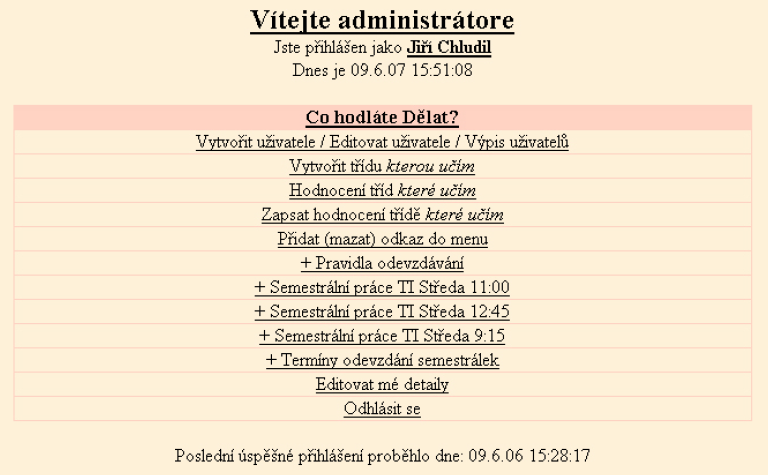
\includegraphics[width=15cm]{figures/jaguI.png}
\caption{Rozhraní cvičícího - Jagu II}
\label{fig:jaguI}
\end{center}
\end{figure}

Hned v následujícím semestru se přišly nové požadavky na podporu cvičení předmětů Teoretická informatika a Aplikace výpočetní techniky. Tyto požadavky zapříčinili nutnost systém v podstatě celý přepsat, bylo nutné přidat například podporu pro zadávání semestrálních prací, zakomponovat bodování docházky a podobně. Nová verze - Jagu 2 - si ovšem stále nesla neduhy svého předchůdce, především co se týče grafické prezentace a přehlednosti. Na základě zkušeností s vývojem těchto dvou verzí došel Jiří Hunka k závěru, že je nutné vyvinout nový systém, který nebude postaven na bázi pouze jednoho předmětu, ale bude univerzální.

První  verze Studentovy Berličky vznikla v rámci bakalářské práce Jiřího Hunky v roce 2007. Vznikl tak komplexní systém, který usnadnil cvičícím vedení agendy cvičení, a studentům poskytl možnost kdykoliv zjistit vlastní hodnocení. Nová verze umožňovala bodování docházky, evidenci bodů za aktivitu na každé hodině, samozřejmě evidenci testů a také hodnocení a odevzdávání semestrálních prací.

\subsection{Současný stav a budoucnost}

Diplomová práce Jiřího Hunky, ve které se zabýval především uživatelským testováním, končí ne zrovna optimistickými slovy: 
\begin{quotation}
Vizí do budoucna je převést vlastní Studentovu berličku v pouhé GUI a
veškeré další činnosti ponechat na databázi. Toto rozvržení by společně
s využitím protokolu SOAP umožnilo kompletní napojení na jakékoli rozšíření, jinou aplikaci či vlastní spojení i s GUI Studentovy berličky.
Ideálním postupem by bylo celou Studentovu berličku napsat znova. Nejedná se pouze o silná slova, ale o ideální postup, který se navrhuje projektům, které dospějí do této fáze.
\end{quotation}

Současný stav Studentovy Berličky je v podstatě typický pro aplikaci napsanou v době, kdy PHP nemělo plnou podporu OOP. Aplikace tak nemá žádnou architekturu, prezentační a aplikační logika jsou úzce spojeny a aplikaci nelze snadno rozšiřovat. Z těchto důvodů bylo rozhodnuto, že bude Studentova berlička bude navržena a vytvořena od základů znovu, ve formě samostatných modulů. Na toto téma již bylo zadáno v minulých semestrech několik bakalářských a diplomových prací, které řeší jednotlivé části (jádro, datové úložiště, podporu pluginů, a několik samostatných modulů).



%*****************************************************************************
\chapter{Popis problému, specifikace cíle}
\label{popis}
V této kapitole je postupně probráno existující řešení získávání dat z KOS Studentovou Beličkou, z jehož nedostatků vyplyne cíl této práce. Následně jsou probrány možnosti, jakými lze získat data z KOS, včetně prozkoumání existujících řešení, a specifikace požadavků na vlastní řešení.  

\section{Současný způsob získávání dat z KOS}
Jak popisuje Jiří Hunka ve své bakalářské práci\cite{hunka:bp}, současná verze Studentovy Berličky používá pro import textové soubory spravované Ing. Martinem Bílým. Ing. Bílý k nim uvádí tyto informace:

\begin{quotation}
Není mi známo, jak vypadají skutečné databázové tabulky KOSu a jaké všechny atributy obsahují. Vycházím z pravidelně exportovaných XML dat v souboru rz.xml, která předzpracovávám, načítám do jiné databáze, lehce začišťuji a podstatné informace ukládám do následujících souborů v podadresáři data. Každý soubor v datovém adresáři představuje jednu tabulku.

K souborům umožním přístup těm, kteří je potřebují pro svůj projekt, diplomovou či i jinou práci. Uživatel se zavazuje, že data použije právě k těmto účelům.
\end{quotation}

Jednotlivé textové soubory obsahují informace o katedrách, místnostech, studentech, učitelích, rozvrhové lístky a zápisy studentů na předměty. Víceméně jde tedy o kompletní rozvrh. Data jednotlivých sloupců jsou v souborech oddělena čárkou, Ing. Bílý uvádí v dokumentaci i jejich významy.

Pro tato data je v databázi Studentovi Berličky vytvořena struktura tabulek, která je obrazem struktury dat v souborech. Import dat pak probíhá ručním spouštěním skriptu administrátorem. Tento skript je v současné verzi spouštěn několikrát, ale pouze na začátku semestru. Několikrát proto, že ve zdrojových datech můžou nějaké záznamy několik dní chybět. V průběhu semestru pak již nedochází k aktualizaci dat, přesuny studentů mezi paralelkami jsou řešeny interně v Berličce a jakákoliv změna v KOS se v semestru už neprojeví.

Spuštění importního skriptu v průběhu semestru by totiž bylo velmi rizikové. Studentova Berlička přímo aktivně používá tabulky s importovanými daty a zapisuje do nich změny, které se provádějí v aplikaci. Spuštění importního skriptu by tak mělo za následek jejich přepsání daty z KOS, které nemusí být správné a přesné (student chodí na jiné cvičení, než kam je zapsán - v Berličce si ho cvičící přesune, v KOSu to například kvůli kapacitě nemusí jít).

Tento způsob má několik zjevných nedostatků:
\begin{itemize}
\item Import není automatický, ale je spouštěn ručně a vyžaduje součinnost s administrátorem.
\item Data se v průběhu semestru neaktualizují. Změny paralelek, zrušení předmětu a podobné změny v KOS se v Berličce neprojeví.
\item Případnou aktualizaci lze řešit jen stylem \uv{buď a nebo}. Bylo by velmi problematické dosáhnout například pouze aktualizace dat uživatelů, ale nepřepsat data o rozdělení paralelek, které mohou být v Berličce odlišná (upravená) od dat v KOS.
\item Bylo by velmi problematické data o rozvrhu poskytnout jiným aplikacím a rozšířením Studentovy Berličky.
\end{itemize}

\section{Cíl práce}
Pro novou verzi Studentovy Berličky je proto nutné připravit nové řešení importu dat z univerzitního systému.

Cílem této práce je toto řešení najít v rámci existujících aplikací, nebo navrhnout a implementovat řešení nové. Toto řešení musí být dostatečně univerzální, aby dokázalo obsloužit požadavky nejen Studentovy Berličky, ale i jejích rozšiřujících modulů a případně dalších nezávislých aplikací, například připravovaného systému na podporu projektů v týmu. Zároveň by nový způsob měl odstranit většinu, ne-li všechny, zmíněné nedostatky.

Výsledný systém by tedy měl umožňovat:
\begin{itemize}
\item Poskytnutí stejného rozsahu dat, jako má stávající řešení.
\item Možnost přístupu ke stále stejné verzi databáze (revizi).
\item Možnost částečné aktualizace revize.
\item Rozhraní, které lze snadno využívat v široké škále aplikací.
\end{itemize}

\section{Možnosti získání dat o rozvrhu}

Studijní informační systém KOS je uzavřený systém, ke kterému v podstatě nelze získat přímý aplikační přístup. Samotný KOS totiž neposkytuje žádné dostupné API, pomocí kterého by mohli aplikace jednotlivých fakult a kateder získat alespoň základní data o studentech, učitelích a vyučovaných předmětech. Někteří si proto v minulosti vyžádali nějakou formu generovaného výstupu vhodnou pro svou aplikaci. Jedním takovým exportem je i soubor rz.xml který obsahuje data rozvrhu, tady studenty, učitele, předměty, zápisy do paralelek a další. Každý, kdo chce tento typ dat ve své aplikaci použít, musí tento soubor nějakým způsobem zpracovat - typicky převést do podoby databáze se kterou pak pracuje samotná aplikace. 

Rozhodl jsem se proto nejdříve zjistit, jak získávání dat řeší jiné aplikace a zda-li by se nedaly nějakým způsobem využít pro Studentovu Berličku.

\subsection{EDUX}
Aplikace EDUX je webový systém sloužící k organizaci výuky a publikování výukových materiálů na webu pro učitele i studenty. Jde o otevřený systém postavený na aplikaci DokuWiki, jejíchž vlastnosti přebírá a rozšiřuje. V současné době je provozován na FEL i FIT na serverových clusterech. Studentova Berlička by měla v budoucnu s EDUXem úzce spolupracovat, stát se v podstatě jeho plug-inem. EDUX samozřejmě také potřebuje pro své fungování data o rozvrhu z KOS, která získává z exportu rz.xml. Požádal jsem proto Ing. Tomáše Kadlece, který se o EDUX stará, o vyjádření jakým způsobem aplikace zmíněný soubor zpracovává.

Zdrojové XML je EDUXem zpracováno pomocí XSL transformace, ze které jsou generovány informace rovnou ve formátu pro Dokuwiki. Tento import je prováděn každou noc, aplikace si zároveň udržuje 90 dní zpět rozdílovou zálohu pro případ problémů, ale jak uvádí Ing. Kadlec, za 1,5 roku provozu EDUXu ji nebylo nutné použít. Studentově Berličce ale nemůže EDUX nabídnout žádný výstup, žádnou \uv{mezi-databázi} vlastně ani nepoužívá.

\subsection{KOS API}
V letním semestru 2009/2010 vytvořil Jakub Jirůtka v rámci své bakalářské práce\cite{jirutka} aplikaci nazvanou KOSapi. Jde o implementaci webové služby na bázi REST architektury nad zmíněným exportem z KOS rz.xml. Tato aplikace významně zjednodušuje získávání dat rozvrhu z KOS, neboť složité parsování a transformaci XML souboru do přístupnější formy nahrazuje RESTful webová služba s jednoduchou komunikací na bázi požadavek-odpověď nad protokolem HTTP.

Ačkoli tato aplikace řeší několik úskalí práce s rz.xml, nakonec jsem ji nepoužil především z těchto důvodů:
\begin{itemize}
\item KOSapi nepodporuje vytváření revizí dat, natož pak jejich porovnávání a částečnou aktualizaci. Bylo by proto nejspíše nutné vytvořit nějakou formu nadstavby nad KOSapi, která by tuto funkcionalitu doplnila.
\item Nejpodstatnější důvod je ale ten, že v době, kdy jsem na této práci začal pracovat (jaro 2010) nebylo KOSapi ještě hotové a nasazené, k tomu došlo až na podzim. Je ovšem možné, že v budoucnu bude KOSapi nějakým způsobem využito.
\end{itemize}

\section{Specifikace požadavků}
Jelikož se mi nepodařilo najít takovou existující aplikaci, která by splnila všechny požadavky a mohla data poskytnout, rozhodl jsem se navrhnout a implementovat vlastní řešení. Prvním krokem k jejímu zdárnému vývoji je přesné specifikování požadavků.
\subsection{Funkční požadavky}

\begin{enumerate}
\item Importér z KOS
\begin{enumerate}
\item Importní modul bude převádět data ze souboru rz.xml do podoby relační databáze.
\item Import bude plně automatický.
\item Importní modul bude kontrolovat referenční závislosti mezi daty.
\item Importní modul nebude závislý na aktuální struktuře rz.xml, ale bude konkrétní strukturu zjišťovat ze samotného souboru.
\item Zpracování bude logováno aby bylo možné odhalit případná selhání.
\end{enumerate}

\item Webová služba
\begin{enumerate}
\item Systém bude poskytovat data prostřednictvím webové služby.
\item Chyby při zpracování požadavků na WS budou logovány.
\end{enumerate}

\item Poskytovaná data
\begin{enumerate}
\item Systém bude umožňovat definici rozhraní služby pro každou klientskou aplikaci.
\end{enumerate}

\item Aktuálnost dat
\begin{enumerate}
\item Pro každou klientskou aplikaci bude možné definovat přístup ke stále stejné revizi databáze.
\item U revize bude možné na úrovni tabulek definovat stupeň udržované aktuálnosti dat (viz kap. \ref{rozbor})
\item Revize může obsahovat pouze podmnožinu celé databáze.
\item Revize bude možné vzájemně porovnávat.
\item Zároveň systém také umožní přístup ke vždy aktuálním datům (každodenně importovaným).
\end{enumerate}
\end{enumerate}

\subsection{Nefunkční požadavky}
\begin{enumerate}
\item Použitelnost
\begin{enumerate}
\item Celá aplikace bude uživatelsky přívětivá a snadno použitelná.
\item Použitá technologie WS umožní integraci služby s aplikacemi na běžně používaných platformách pro vývoj webových aplikací a plug-inů Studentovy Berličky (PHP, C++, Java...).
\end{enumerate}

\item Modulárnost
\begin{enumerate}
\item Celá aplikace se bude skládat z oddělených modulů pro import rz.xml, zpracování požadavků WS a samotné administrace.
\item Moduly na sobě nebudou závislé a nahrazení jednoho modulu by nemělo ovlivnit ostatní.
\end{enumerate}

\item Přístupová práva
\begin{enumerate}
\item Aplikace nebude řešit práva přístupu do administrace služby, to je záležitost webového serveru a nadřazených aplikací.
\item Bude však implementovat nějakou formu identifikace, případně i autorizace klientských aplikací při komunikaci přes WS.
\end{enumerate}

\item Nezávislost na databázi
\begin{enumerate}
\item Systém nebude svázán s konkrétní relační databází.
\end{enumerate}

\end{enumerate}

\subsection{Rozbor požadavků} \label{rozbor}
Některé výše zmíněné požadavky vycházejí ze zkušeností v provozu aktuální verze Studentovy berličky. V této části bych proto rád specifikoval, proč jsou některé požadavky nutné a důležité.

\subsubsection{Verzování dat a porovnávání revizí}
V exportu rz.xml se čas od času vyskytují chyby. To je zkrátka potřeba brát jako fakt a počítat s ním. Jak jsem se dozvěděl od Ing. Chludila a Ing. Kadlece, občas se například stane, že část dat v exportu několik dní chybí a poté se v něm zase objeví. V minulosti také došlo k přečíslování identifikátorů studentů, což způsobilo nefunkčnost Studentovy Berličky, která je samozřejmě v databázi využívá. Základním požadavkem na novou aplikaci tedy je, aby dokázala předejít těmto situacím.

To by mělo být zajištěno právě možností vytvářet revize databáze. Každá tabulka v revizi také bude mít možnost definovat stupeň zpracování aktualizace:
\begin{itemize}
\item Neaktualizovat - V tomto případě zůstane tabulka stále stejná z okamžiku vytvoření revize.
\item Aktualizovat pouze data
\item Aktualizovat vše - to znamená strukturu tabulky i data
\end{itemize}

Typickým příkladem proč jsou tyto možnosti potřeba je tento - student si v KOS změní například e-mail a my samozřejmě chceme, aby se změna objevila i v Berličce. Zároveň ale nechceme, aby se u tabulky samovolně mohla změnit struktura a proto nechceme tyto data získávat přímo z \uv{živé} databáze. Správa revizí a jejich aktualizací by také měla pomoci předejít zmíněnému problému s přeindexováním dat.

\subsubsection{Vytváření podmnožin databáze}
Nutnost tohoto požadavku plyne z prostého faktu, že databáze vytvořená ze současného rz.xml obsahuje cca 130 000 záznamů a zabírá cca 30 MB. Typická klientská aplikace ale nepotřebuje všechna data, ale jen jejich část, například informace o jednom předmětu a jeho studentech. Z toho důvodu je zbytečné vytvářet revizi celé databáze, ale stačí nám pouze její část. U této části musí být také zajištěna konzistence dat , neboť tabulky jsou vzájemně propojeny cizími klíči. Tomuto problému se budu podrobněji věnovat déle v textu.

\subsubsection{Vlastní definice rozhraní}
Ze zkušenosti vím, že definice univerzálního rozhraní služby je velmi problematická. Vždy totiž časem přijde takový požadavek, který stávající rozhraní buď vůbec neřeší, nebo jej řeší neefektivně. Takový požadavek pak typicky vyústí v přidání dalších parametrů nebo rovnou nových operací služby, a to \uv{jediné, správné a univerzální} rozhraní se rozrůstá do velkého objemu, a stává se nepřehledným.

Tomu jsem se chtěl vyhnout, proto místo jediného rozhraní aplikace bude umožňovat definici vlastního rozhraní webové služby unikátně pro každou klientskou aplikaci.


%*****************************************************************************
\chapter{Analýza}

Jak už jsem naznačil, aplikace využije jako zdroj dat soubor rz.xml. Tato kapitola obsahuje analýzu dat ze zdrojového souboru včetně popisu významu jednotlivých elementů, které se v něm vyskytují. Taktéž v této kapitole najdete možné varianty systému verzování databázových dat.

\section{Struktura exportu z KOS}
Práce s rz.xml je celkem obtížná, protože k němu neexistuje naprosto žádná dokumentace. U většiny elementů a atributů lze ale celkem bez problémů rozluštit jejich význam, a tak jsem v podstatě až do doby, než Jakub Jirutka\cite{jirutka} dokončil svou práci neměl potřebu pátrat po významu těch několika zbylých, nerozluštěných. V své práci Jakub Jirůtka zpracoval velmi podrobný popis struktury souboru, a vytvořil tak \textit{de facto} jeho první dokumentaci. 

Soubor obsahuje jeden kořenový element ROZVRH, v něm pak následují elementy jednotlivých \uv{tabulek}, každý s právě jením výskytem. Tabulky pak obsahují data jednotlivých \uv{řádků}, názvy atributů jsou sloupce, hodnoty atributů pak data jednotlivých sloupců. Některé elementy řádků pak ještě obsahují vnořené elementy, kde pak platí že název tagu je názvem sloupce, data v něm pak data příslušného sloupce. Jde například o popis předmětu a požadavků u tabulky PREDMETY, tedy o delší text.

Následující text popisuje strukturu rz.xml, zaměřil jsem se především na rozdíly oproti struktuře kterou popisuje Jakub Jirutka ve své práci\cite{jirutka}. Jednotlivé elementy nejsou v následujícím textu uvedeny v pořadí v jakém se nacházejí v exportu, ale podle logických souvislostí.

\subsection{ROZVRH}
Element ROZVRH je kořenovým elementem XML stromu dokumentu. Obsahuje základní informace o semestrech:
\begin{itemize}
\item \texttt{semestr, aktsem, aktsem2} - Kódy semestrů pro které se jsou data v rz.xml generována. V průběhu semestru je ve všech atributech uvedený stejný kód (např. B101), v době kdy se tvoří rozvrh se kódy různí.
\item \texttt{nazev\_semestru} - Textový název aktuálního semestru (odpovídá semestru v atributu \texttt{semestr})
\item \texttt{zacatek\_sem, konec\_sem} - Obsahuje datum začátku, resp. konce aktuálního semestru dle harmonogramu školního roku. Formát data je \texttt{dd.mm.yyyy}.
\end{itemize}

\subsection{KATEDRY}
V databázi KOS tvoří jsou rektorát, fakulty a katedry umístěny v jedné tabulce a tvoří stromovou strukturu středisek. Záznamy jsou spojeny relací \texttt{nadrizena=id}, přičemž fakultu od katedry lze snadno rozlišit tím, že fakulta má nadrizena=1 (id rektorátu). V souboru rz.xml nalezneme ale jen FEL a jeho katedry, takže tuto relaci nemůžeme explicitně přenést do databáze.

Element obsahuje atributy \texttt{id, nadrizena, nazev\_cz, nazev\_en} (český a anglický název) a číselný \texttt{kod} střediska.

\subsection{MISTNOSTI}
Element obsahuje místnosti ve kterých probíhá výuka. Atributy jsou \texttt{id, cislo} (např. KN:E-107), lokalita (\texttt{lok}) a odkaz na katedru, která má místnost ve správě (\texttt{kat\_id}).

\subsection{PREDMETY}
Element PREDMETY obsahuje všechny vypsané předměty v semestrech uvedených v elementu ROZVRH. Protože jsou samozřejmě stejné předměty vypisovány v různých semestrech, jsou jednotlivé záznamy identifikované složeným primárním klíčem \texttt{id, sem\_id}.

Element obsahuje následující atributy a elementy:

\begin{itemize}
\item \texttt{id, sem\_id} identifikátor záznamu
\item \texttt{kod} Kód předmětu, např. Y36BAP.
\item \texttt{garanti} Identifikátory učitelů, kteří jsou garanty předmětu. Hodnoty jsou oddělené čárkou.
\item \texttt{kat\_id, pr\_kat\_id} Identifikátor katedry, která předmět zajišťuje (oba atributy obsahují stejnou hodnotu).
\item \texttt{nazev, nazev\_an} Český, respektive anglický název předmětu (anglický název má skutečně suffix \textit{an}, nikoliv \textit{en})
\item \texttt{rozsah} Hodinová dotace předmětu.
\item \texttt{pr\_forma\_studia} Forma studia pro kterou je předmět určen.
\item \texttt{pr\_kredity} Počet kreditů za absolvování předmětu.
\item \texttt{pr\_zpuszak} Způsob zakončení předmětu, hodnoty [KZ|Z|ZK|Z,ZK|NIC].
\item \texttt{pr.kapacita, pr\_obsazeno, pr\_zapnuto} Kapacita předmětu, počet zapsaných a příznak určující, zda-li je zapnuto hlídání překročení kapacity. ( atribut kapacita skutečně obsahuje v názvu tečku, nikoliv podtržítko).
\item \texttt{pr\_program\_id} ID programů ve kterých je možné předmět zapsat. Obsahuje hodnoty oddělené čárkou.
\item \texttt{pr\_p\_blok, pr\_c\_blok, pr\_l\_blok} Toto jsou pomocné atributy, které určují, kolik rozvrhových lístků má být vygenerováno pro přednášky, cvičení a laboratoře.
\item \texttt{pozadavky, poznamka} Toto jsou vnořené elementy v elementu řádku, obsahují textový popis požadavků na předmět, respektive textovou poznámku.
\end{itemize}
Na rozdíl od toho, co popisuje Jakub Jirůtka, v současném rz.xml se nevyskytuje atribut \texttt{pr\_znamky\_hlas}.

\subsection{Učitelé a studenti}
V KOSu existují samostatné tabulky osob, učitelů a studentů. V exportu jsou ovšem data osoby a učitele, resp. studenta sloučeny do jednoho elementu, což může přinést určité problémy.

\subsubsection{UCITELE}
U učitelů existuje jen drobná záludnost, a to že někteří externí učitelé, kteří nemají přístup do KOS nemají vyplněný atribut \texttt{login}. Element obsahuje tyto atributy:
\begin{itemize}
\item \texttt{id}
\item \texttt{kat\_id} Identifikátor katedry, ke které učitel patří. Obsahuje i katedry, které v elementu \texttt{KATEDRY} nejsou, a také mnoho \texttt{NULL} hodnot.
\item \texttt{login}
\item \texttt{jmeno, prijmenu, titul\_pred, titul\_za}
\item \texttt{uc\_email} Obsahuje nevalidní e-maily a množství nevyplněných hodnot.
\item \texttt{osobni\_cislo}
\item \texttt{osoba\_eid}
\end{itemize}

\subsubsection{STUDENTI}
Záznamy v této části jsou identifikovány složeným klíčem \texttt{id, stud\_id} (id studia). Jedna osoba totiž může být zapsána do několika studijních oborů najednou.
Element obsahuje tyto atributy:

\begin{itemize}
\item \texttt{id, stud\_id} identifikátor záznamu
\item \texttt{jmeno, prijmeni, titul, titul\_za} Celé jméno včetně titulů (všimněte si, že na rozdíl od záznamů učitelů nemá titul před jménem suffix).
\item \texttt{obor} Textový název studijního oboru, např. \uv{Web a multimedia (bakalářský)}
\item \texttt{osoba\_eid}
\item \texttt{osoba\_id} Obsahuje stejné hodnoty jako atribut \texttt{id}
\item \texttt{rocnik}
\item \texttt{skupina} Studijní skupina
\item \texttt{stud\_email}
\item \texttt{stlan\_id} ID studijního plánu
\end{itemize}

\subsection{ZAPISY\_PREDMETU}
Obsahuje data spojové tabulky pro zápisy studentů do předmětů. Obsahuje celý identifikátor předmětu \texttt{predmet\_id, sem\_id} a identifikátor studenta \texttt{student\_id}.

\subsection{LISTKY}
Element LISTKY obsahuje záznamy o vypsaných paralelkách přednášek a cvičení přiřazených do konkrétních dní, časů a místností. Existují zde rozvrhové lístky předmětů a pak speciální události jiného typu - například porady, semináře, výuka na jiných školách a podobně. Tyto speciální záznamy lze rozlišit tím, že atribut \texttt{typ\_vyuky} obsahuje hodnotu \uv{J}. V tomto elementu najdeme tyto údaje:
\begin{itemize}
\item \texttt{id}
\item \texttt{den\_cis} Den v týdnu, rozsah 1-7.
\item \texttt{hodina} Číslo vyučovací hodiny, kdy lístek začíná.
\item \texttt{pocet\_hodin} Počet vyučovacích hodin lístku.
\item \texttt{katedra1\_id} Katedra, která vlastní lístek.
\item \texttt{katedra2\_id} Katedra, která zajišťuje výuku.
\item \texttt{mistnost\_id} Místnost, kde se výuka probíhá.
\item \texttt{typ\_vyuky} Identifikace, zda jde o přednášku (P), cvičení (C), laboratoř (L), nebo speciální jinou událost (J).
\item \texttt{pno, cno, lno} Jde o identifikátory ke které paralelce lístek přísluší. Např. \texttt{pno=1, cno=202, lno=NULL} znamená, že paralelku cvičení 202 lze zapsat jen s přednáškovou paralelkou 1.
\item \texttt{predmet\_id} ID předmětu, ke kterému lístek přísluší. Element lístky neobsahuje druhou část složeného klíče předmětu \texttt{sem\_id}, protože se exportují jen lístky k semestru uvedeném v atributu \texttt{semestr} elementu \texttt{ROZVRH}.
\item \texttt{ucitel1\_id, ucitel2\_id} ID učitelů, kteří zajišťují výuku. Pokud jde o lístek typu jiná událost, je vyplněn pouze \texttt{ucitel1\_id} a jde v tomto případě o vlastníka události.
\item \texttt{sudy\_lichy} Příznak, zda-li jde o lístek, který je platný liché nebo sudé týdny (pokud vždy, obsahuje atribut \texttt{NULL}).
\item \texttt{text} U speciálních jiných událostí obsahuje její popis.
\item \texttt{paralelka\_kod}
\item \texttt{par\_jmeno} Jméno paralelky, většinou obsahuje nějakou poznámku.

\end{itemize}

\subsection{LISTKY\_STUDENTU}
Obsahuje data spojové tabulky pro zápisy studentů do rozvrhu. Obsahuje identifikátor lístku \texttt{listek\_id} a identifikátor studenta \texttt{student\_id}. Mimochodem jde o datově největší element v exportu.

\subsection{JEDNORAZOVE\_TERMINY}
Tento element obsahuje informace o jednorázových akcích, která se například používají pro hromadné kontroly semestrálních prací nebo udělování zápočtů.

Najdeme zde tyto atributy:
\begin{itemize}
\item \texttt{id}
\item \texttt{nazev} Název akce
\item \texttt{datum, cas} Datum a čas konání akce.
\item \texttt{fakulta\_id}
\item \texttt{katedra\_id}
\item \texttt{misto\_id}
\item \texttt{predmet\_id, sem\_id} Identifikátor předmětu, kterého se akce týká.
\item \texttt{kapacita, obsazeno} Kapacita akce a počet přihlášených.
\item \texttt{uzaverka} datum uzavření přihlašování (dd.mm.yyyy).
\item \texttt{vypsal\_id}
\item \texttt{poznamka}
\end{itemize}

\subsection{ZAPISY\_JA}
Obsahuje data spojové tabulky pro zápisy studentů na jednorázovou akci. Obsahuje identifikátor akce \texttt{termin\_id} a identifikátor studenta \texttt{student\_id} a \texttt{id}.

\subsection{VYPSANE\_TERMINY}
Element obsahuje vypsané termíny zkoušek k předmětům. Najdeme v něm následující atributy:

\begin{itemize}
\item \texttt{id}
\item \texttt{vypsal\_id} 
\item \texttt{zacatek} Datum a čas začátku termínu (formát dd.mm.yyyy HH:MM)
\item \texttt{konec} Datum a čas konce termínu (formát dd.mm.yyyy HH:MM)
\item \texttt{predmet\_id, sem\_id} Identifikátor předmětu
\item \texttt{misto\_id} ID místnosti, kde by se termín měla konat. Často není vůbec vyplněné a skutečná místnost je uvedená v poznámce.
\item \texttt{poznamka}
\end{itemize}

\subsection{ZKOUSEJICI}
Obsahuje data spojové tabulky určující, kteří učitelé předmět zkouší. Obsahuje identifikátor předmětu \texttt{predmet\_id, sem\_id} a identifikátor učitele \texttt{osoba\_id}.

\subsection{CASOVA\_OKENKA}
Tento element obsahuje data okének, které se používají pro plánování rozvrhu. Vždy když je vytvořena nějaká akce (např. lístek) označí se místnost jako zabraná právě vytvořením časového okénka. Žádný jiný element v exportu ale neobsahuje odkaz na záznamy v tomto elementu a ani tento element neobsahuje identifikaci místnosti ke které se vztahuje. Jeho existence tedy naprosto postrádá smysl.

Element obsahuje atributy \texttt{id}, datum ve formátu dd.mm.yyyy (\texttt{den}), času začátku a konce okénka (\texttt{zacatek}, \texttt{konec}) a poznámku (\texttt{poznamka}).

\section{Verzování databáze}
Vzhledem ke způsobu získávání data a požadavkům na systém přicházejí pro verzování dat z KOS pouze dva možné způsoby - uchovávání rozdílů a plné kopírování databází.

\subsection{Rozdílová revize}
Tento způsob spočívá v tom, že existuje jedna databáze která obsahuje všechny data a vytvoření a aktualizace pak probíhá formou uchování rozdílů oproti hlavní databázi. Výhodou tohoto postupu je malá náročnost na velikost úložiště, protože hlavní databáze existuje jen jednou a ostatní databáze revizí obsahují pouze záznamy, které se změnily. Další výhodou je jednodušší implementace aktualizací revizí, především v případě, kdy se příslušná tabulka má aktualizovat včetně struktury (v takovém případě by klient přistupoval nejspíše přímo k datům v hlavní databázi).

Velkou nevýhodou je ovšem rychlost. Data by se musela při požadavku webové služby získávat z hlavní databáze a zároveň by se na ně musely aplikovat rozdíly uchované v záznamech revize, což by způsobilo vyšší výpočetní náročnost služby. Z toho důvodu jsem tento způsob nepoužil.

\subsection{Kopírování verzí}
Při použití tohoto způsobu dojde při vytvoření k přímému zkopírování dat do revize. Webové služba se pak při vyhledávání výsledků dotazuje pouze jednoho datového zdroje a její implementace tak je podstatně jednodušší než u předchozí varianty. Tento způsob má jednoznačnou výhodu v rychlosti, požadavky na WS se jednoduše čtou data z jedné databáze. Nevýhodou pak je větší náročnost na velikost úložiště a komplikovanější způsob aktualizace revizí. 

Pro implementaci aplikace jsem zvolil tuto variantu, především kvůli jednodušší implementaci obsluhy webové služby a tím i pravděpodobně vyšší rychlosti zpracování požadavků. Vzhledem k umožnění tvorby revizí, které neobsahují celou databázi, ale jen její podmnožinu, by neměl být problém ani s větší datovou náročností řešení oproti rozdílovým revizím.


%*****************************************************************************
\chapter{Návrh řešení}

V této kapitole naleznete seznámení s technologiemi, které byly použity při zpracování této práce. Dále je zde popsán princip zpracováni importu, a řešení verzování dat a vlastní definice rozhraní webové služby.

\section{Použité technologie}
Pro implementaci aplikace byl použit skriptovací jazyk PHP a databázový stroj MySQL, a to především z toho důvodu, že s nimi mám nejvíce praktických zkušeností. Nezanedbatelným argumentem je také to, že Studentova Berlička je na nich také postavena.

\subsection{PHP}
PHP je velmi oblíbený skriptovací programovací jazyk používaný především pro tvorbu dynamických webových stránek. Od verze 5 disponuje také dobrou podporou objektově orientovaného programování. Přestože si jazyk s sebou z minulosti nese spoustu nevýhod, jde dnes nejspíše o nejpoužívanější jazyk pro tvorbu webů. Poslední významná verze PHP 5.3 rozšířila možnosti jazyka také o deklaraci jmenných prostorů, anonymní funkce, řetězení výjimek a mnoho dalších menších změn.

\subsection{MySQL}
MySQL je multiplatformní relační databázový systém od švédské společnosti MySQL AB. Pro svou jednoduchou instalaci, konfiguraci, výkon a také proto, že je volně dostupné pod GNU GPL, je na webových serverech velmi oblíbená, především v kombinaci s Apache a PHP. MySQL bylo od počátku svého vývoje optimalizováno především pro výkon, a to i za cenu zjednodušení funkčnosti, například podpora definice cizích klíčů a transakcí byla přidána až ve verzi 3.23, šest let od prvního vydání. MySQL podporuje většinu ze standartu SQL:99, doplněnou, stejně jako u většiny ostatních DBMS, o vlastní rozšíření.

\subsection{Nette Framework}
Nette je český framework pro tvorbu webových aplikací v PHP 5. Zaměřuje se především na eliminaci bezpečnostních rizik a vede programátory k čistému návrhu aplikace s důrazem na budoucí rozšiřitelnost. Využívá událostmi řízeného programování a principy třívrstvé architektury Model-View-Presenter, DRY\footnote{neopakovat se} a KISS\footnote{řešit vše jednoduše}. Mezi jeho silné stránky patří také výkonný nástroj pro odchytávání chyb (Nette\verb|\|Debug), který místo prosté textové informace PHP zobrazí celou stránku s detailním výpisem místa, kde k chybě došlo, call stacku a důležitých proměnných aplikace. Dalšími velmi užitečnými částmi frameworku jsou formuláře se silným validačním jazykem, routování, které slouží jak pro zpracování požadavků, tak i pro generování odkazů, a v neposlední řadě šablonovací jazyk Latte.

Za dva roky veřejné existence si Nette získalo velkou popularitu na česko-slovenském webu, včetně komerčních aplikací. Původním autorem Nette je David Grudl, dnes se o jeho vývoj stará komunita vývojářů Nette Foundation. Framework je volně dostupný pod licencí GNU/GPL a licencí Nette, která je obdobou BSD licence\cite{nette:licence}.

\subsection{Databázová abstrakce}
Nutnost použití databázové abstrakce plyne z NP4a. Přímo v distribučním balíku PHP najdeme rozšíření PDO, které poskytuje abstrakční vrstvu a odstínění od konkrétní databáze. Já jsem se rozhodl nepoužít přímo PDO, ale knihovnu dibi.
\subsubsection{dibi}
Dibi je, jak se dočteme v podtitulu názvu \uv{tiny 'n' smart database layer} (malá a chytrá databázová vrstva). Jde o knihovnu, jejímž hlavním cílem je zjednodušit zápis SQL příkazů a ulehčit rutinní úlohy programátora, například získání výsledků jako dvourozměrné pole, vytvoření pole výsledků indexovaného podle klíče z databáze a podobně. Dibi také pomáhá předcházet zranitelnosti webů SQL Injection\footnote{Zranitelnost aplikací podsunutím části nebo celého SQL dotazu přes neošetřený uživatelský vstup.}, neboť všechny parametry, které do dotazů vstupují jsou automaticky escapovány syntaxí podle použité databáze. Lze ho použít jednak jako nadstavbu PDO, tak přímo s nativními PHP rozšířeními pro jednotlivé databázové stroje.
\label{idatabasemanager}
\subsubsection{Rozhraní pro správu databází}
PDO i dibi poskytují abstrakci, která je dostačující pro běžnou aplikaci, které pracuje s jednou databází\footnote{Databází zde myslím kolekci tabulek. U MySQL se používá termín databáze, například u PostgreSQL by byl správný termín \uv{schéma}}. S jinými databázemi lze samozřejmě pracovat prostřednictvím \uv{tečkové} notace {\tt databáze.tabulka.sloupec}, ovšem v momentě, kdy je potřeba nastavit některou databázi jako výchozí (např. u MySQL příkazem {\tt USE database}), nenabízí PDO ani dibi žádnou možnost. Totéž pak platí i pro možnosti pro vytváření databáze a tabulek, jejich mazání, úpravy struktury a podobně.  A to je přesně to, co v této aplikaci potřebuji, neboť každá revize odpovídá samostatné databázi. Přímé zapsání těchto příkazů by samozřejmě způsobilo svázání aplikace s konkrétním DBMS, neboť syntaxe těchto příkazů je u jednotlivých strojů různá.

Z toho důvodu jsem v aplikaci vytvořil jednoduché rozhraní {\tt IDatabaseManager} které odstiňuje ostatní části od specifik databázového stroje. Převod systému pod jiný databázový stroj tedy spočívá jen v implementaci tohoto rozhraní pro konkrétní DBMS a změnu jednoho řádku v konfiguračním souboru.

\subsection{Webové služby}
Webové služby jsou technologický systém, který umožňuje propojit libovolné aplikace na různých platformách pomocí široce podporovaného a vždy dostupného protokolu HTTP. V dnešní době jsou běžně používány dva způsoby implementace webových služeb - REST a SOAP.

\subsubsection{REST}
Architektura REST (Representational State Transfer) zažila v posledních letech obrovskou vlnu popularizace. Není to vlastně ani standart, ale jen architektura rozhraní. Na rozdíl od procedurálního SOAP je REST orientován datově. Každý datový zdroj má specifické URI a pro komunikaci se službou se využívají metody protokolu HTTP GET, POST, PUT a DELETE. Díky tomu jsou REST služby snadno škálovatelné a jednoduché na pochopení. Velkou nevýhodou ovšem je chybějící podpora na úrovni programovacích jazyků (na rozdíl od SOAP).


\subsubsection{SOAP}
SOAP (Simple Object Access Protocol) vychází ze specifikace XML-RPC a přebírá jeho hlavní rys - formát přenášených zpráv a jeho platformní nezávislost. SOAP umožňuje zasílání XML zpráv mezi dvěma aplikacemi a pracuje tedy na principu peer-to-peer. Mnohem častěji se ale technologie používá jako vzdálené volání procedur (RPC), tedy ve schématu klient-server. Stejně jako REST probíhá komunikace nejčastěji protokolem HTTP, ačkoli specifikace protokol nijak nepředepisuje a lze použít i SMTP, FTP a jiné.

Dalším hlavním rysem služby na principu SOAP je možnost definice jejího rozhraní pomocí WSDL schématu. To popisuje procedury, která služba nabízí, typy jejich parametrů a návratových hodnot. I když je zpřístupnění WSDL popisu velmi užitečné a praktické, není vyžadováno a služba může být využívána i bez něj.

Protože na rozdíl od REST existuje v distribuci PHP knihovna pro práci se SOAP, a protože některé již existující části nové Studentovy Berličky SOAP používají, zvolil jsem pro webovou službu také tento protokol.

\section{Architektura aplikace}
Jak jsem již uvedl v části o použitých technologiích, aplikace je postavena na Nette Frameworku, který využívá třívrstvou architekturu Model-View-Presenter. V této části najdete, co je to vlastně návrhový vzor MVP a jeho rozdíly oproti známějšímu vzoru Model-View-Controller.

\subsection{Model-View-Controller}
Model-View-Presenter (dále jen MVP) je odvozený od mnohem známějšího návrhového vzoru Model-View-Controller (dále jen MVC). MVC definuje rozdělení aplikace do tří samostatných vrstev tak, že modifikace v jedné vrstvě má minimální vliv na vrstvy ostatní. Aplikace se rozdělí na:
\begin{itemize}
\item Model - je doménově specifická reprezentace informací, s nimiž aplikace pracuje. V běžné webové aplikaci se modelová část stará o komunikaci s databází a persistenci dat.
\item View (pohled) - jde o část aplikace, se kterou komunikuje uživatel, u webové aplikace jde tedy o šablony a výsledný HTML kód který se zobrazuje v prohlížeči.
\item Controller (řadič, ovladač) - reaguje na události (většinou pocházející od uživatele), a zajišťuje změny v pohledu a v modelu
\end{itemize}
\begin{figure}[h]
\begin{center}
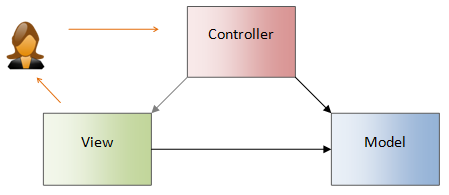
\includegraphics[width=10cm]{figures/mvc.png}
\caption{Architektura Model-View-Controller}
\label{fig:mvc}
\end{center}
\end{figure}
Tento princip poprvé popsal Trygve Reenskaug v roce 1979\cite{mvc-original}. Základní myšlenkou MVC je tedy rozdělení aplikace do tří modulů. Model pouze poskytuje své rozhraní a neví nic o Controlleru ani o View. View o modelu také vědět nemusí (pasivní view), nebo naopak může získávat data přímo z něj, dle zvolené koncepce. Controller potom slouží k propojení zbývajících dvou částí a zpracování požadavků od uživatele.

MVC ovšem nelze chápat dogmaticky. Už v době svého vzniku bylo jeho pojetí velmi různorodé, první návrh vlastně ani není MVC, ale MVCE, kde \uv{E} znamená Editor. K čemu slouží? Jde v podstatě o totéž, co bylo v první implementaci MVC označeno jako Controller a je dokonce společně s View reprezentováno jednou třídou. Ve své prapůvodní podobně MVC vlastně nepoužívá nikdo, role a vztahy jednotlivých vrstev se chápou velmi volně. To je také důvod, proč se Nette Framework hlásí k MVC jen jako k duševně spřízněné architektuře.

\subsection{Model-View-Presenter}

Mnohem výstižnější pro logiku Nette Frameworku je méně známý vzor Model-View-Presenter. V Nette totiž platí myšlenka \uv{nechť je odkaz totéž, co zavolání funkce}\cite{zdrojak:nette}. View už není prostý HTML kód jako na počátku, ale jeho součástí je také Javascript pro obsluhu uživatelských požadavků a AJAXu. Presenter je tedy volán z View, nikoli přímo uživatelem. Došlo tak oproti MVC k posunutí významu vrstev:
\begin{figure}[h]
\begin{center}
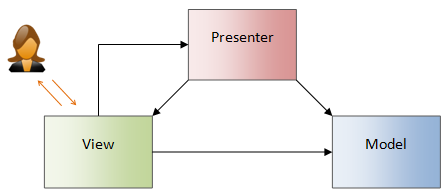
\includegraphics[width=10cm]{figures/mvp.png}
\caption{Architektura Model-View-Presenter}
\label{fig:mvp}
\end{center}
\end{figure}
\begin{itemize}
\item Model se stará stále o to samé, tedy o persistenci dat.
\item View navíc oproti MVC zpracovává uživatelský vstup. Typicky například po kliknutí na odkaz volá nějakou funkci Presnteru. Aplikační logika ve View je většinou chybou.
\item Presenter obsluhuje požadavky z View a manipuluje s Modelem. Spará se vlastně o \uv{prezentování} výsledků (odtud název Presenter).
\end{itemize}

Reálně je problém rozlišit, jestli má aplikace architekturu MVC nebo MVP, protože fakticky se vzory liší jen v detailech. Nette používá označení Presenter, naproti tomu například v Zend Frameworku najdeme Controllery, které mají obdobnou funkčnost. Další informace o MVP lze najít například v \cite{mvp}.

\subsection{Modulární struktura}
Jak vyplývá z NP2, výsledná aplikace má sestávat ze samostatných modulů pro import rz.xml, administraci služby a samotné webové služby. Samotné webové rozhraní administrace je, jak jsem už zmínil, postaveno na MVP frameworku Nette. Importní skript je pak spouštěn samostatně prostřednictvím CLI rozhraní PHP, webová služba je v podstatě jen obslužná třída, které předává požadavky interní PHP třída SoapServer. Importní a WS modul využívá z Nette jen systém automatického načítání tříd, všechny moduly pak sdílí samozřejmě databázové úložiště.

\begin{figure}[h]
\begin{center}
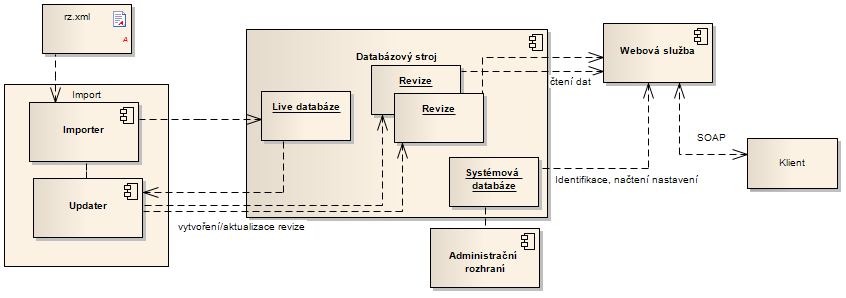
\includegraphics[width=13cm]{figures/struktura.png}
\caption{Schématické znázornění aplikace}
\label{fig:struktura}
\end{center}
\end{figure}

Schéma práce aplikace je znázorněno na obrázku \ref{fig:struktura}. Vstupní XML soubor je zpracován importérem do \uv{live} databáze. Po dokončení samotného importu je spuštěna druhá fáze - aktualizace, případně vytvoření, revizí. Nastavení jejich aktualizace a vytváření se provádí v administrační části, a po vytvoření a nadefinování procedur webové služby jsou data přístupná prostřednictvím samotné webové služby.


\section{Zpracování XML exportu}
Dávkové zpracování velkého množství dat z XML souboru do relační databáze, jejichž aktuální strukturu vlastně zjišťujeme za běhu, a zároveň splnit všechny funkční i nefunkční požadavky a také dosáhnout přiměřené rychlosti zpracování a paměťové náročnosti představovalo nesnadný úkol.

\subsection{Způsob čtení dat}
Pro práci s XML poskytuje PHP (ve verzi 5) hned několik možných přístupů - SimpleXML, SAX, DOM, XPath, XSL transformaci a XMLReader\cite{kosek:phpAxml}. Ze zkušenosti jsem zavrhl SimpleXML, protože je na tento ukol příliš \uv{simple} (hodí se spíše pro jednodušší úlohy) a poté také XPath a XSLT, protože použití jednoho z těchto přístupů by znamenalo rozdrobení funkční logiky do dvou odlišných jazyků. Zbývalo tedy rozhodnutí, zda použít DOM nebo SAX.

\subsubsection{DOM}
Rozhraní DOM je standardizovaný způsob práce s XML dokumenty definovaný W3 konsorciem. Při přístupu přes DOM se z dokumenty v paměti vytvoří hierarchický objektový model, který pak můžeme volně procházet. Každý element, atribut, textový uzel odpovídá v paměti objektu. Pomocí metod a vlastností každého z nich můžeme snadno zjišťovat význam uzlu ve stromu, jeho název, obsah, jeho dětské uzly a uzel rodiče. Strom je možné procházet a vyhledávat v něm. Tento přístup má ale jednu zásadní nevýhodu - pro vytvoření stromu je nutné celý dokument načíst a udržovat v paměti, takže nároky na ni jsou velké.
\begin{figure}[h]
\begin{center}
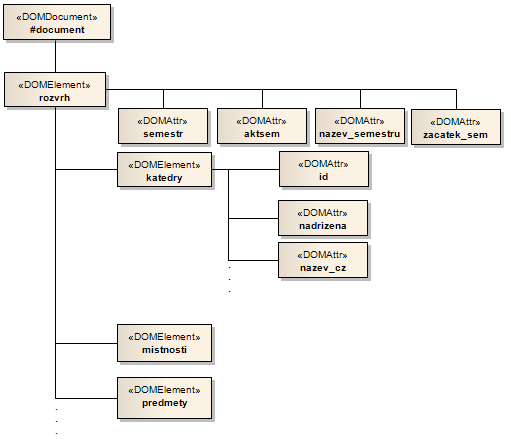
\includegraphics[width=12cm]{figures/dom.png}
\caption{Část DOM stromu souboru rz.xml}
\label{fig:dom}
\end{center}
\end{figure}

První nekompletní verze importéru používala právě objektový přístup pomocí DOM, neboť se mi toto řešení zdálo jednodušší než ostatní přístupy. Tato první verze ovšem pouze převáděla data do databáze tak jak byly, bez jakékoliv kontroly referenčních závislostí. Při snaze tuto funkčnost doplnit jsem ovšem narazil na problém právě s alokací paměti, kdy skript snadno překračoval limit 256 MB zabrané paměti. Taktéž rychlost nebyla nijak oslnivá a tak nezbylo nic jiného, než importní skript navrhnout znovu.

\subsubsection{SAX a XMLReader}

SAX (Simple API for XML) je jednoduché rozhraní, které proudově čte XML dokument a aplikaci předává informace vyvoláváním událostí, které odpovídají částem dokumentu (tzv. push model). Díky tomu je zpracování rychlé a paměťově nenáročné, na druhou stranu je jeho implementace v porovnání s jinými přístupy komplikovanější. Specifikem implementace SAX v PHP je také to, že rozhraní není tak rychlé jako v jiných jazycích, protože má velkou režii předávání dat mezi samotným parserem v C a aplikací v PHP. 

\begin{figure}[h]
\begin{center}

\includegraphics[width=12cm]{figures/sax.png}
\caption{Rozhraní SAX - princip push modelu}
\label{fig:sax}
\end{center}
\end{figure}

Je proto většinou mnohem vhodnější použít třídu XMLReader, což je implementace pull modelu na bázi rozhraní SAX. Data ze zpracovávaného dokumentu tak čteme až v momentě, kdy je aplikace potřebuje a výsledný kód je mnohem jednodušší a přímočařejší. Navíc XMLReader je, na rozdíl od procedurálního SAX, v PHP implementován objektově, což práci s ním ještě více usnadňuje.

\begin{figure}[h]
\begin{center}

\includegraphics[width=12cm]{figures/xmlreader.png}
\caption{Rozhraní XMLReader - princip pull modelu}
\label{fig:xmlreader}
\end{center}
\end{figure}


\subsection{Hlídání referenční integrity}

Najít správné řešení kontroly referenčních závislostí dat při splnění funkčních požadavků 1c a 1d vyžadovalo přistoupit k určitým kompromisům. Je totiž prakticky nemožné rozeznat přímo ve struktuře rz.xml atributy které jsou cizími klíči a správně je navázat na odpovídající záznamy. 

\subsubsection{Definice referencí} \label{defref}
Z toho důvodu jsem po konzultaci s vedoucím práce přistoupil k řešení, kdy aplikace umožňuje definici referenčních závislostí prostřednictvím webového formuláře v administračním rozhraní. Prostřednictvím tohoto jednoduchého formuláře je možné nadefinovat nejen cizí klíče, ale i primární klíče a obecné databázové indexy.

\begin{figure}[h]
\begin{center}
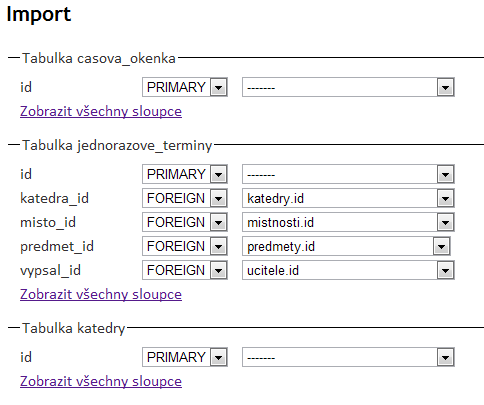
\includegraphics[scale=0.6]{figures/import_setup.png}
\caption{Ukázka rozhraní pro definici klíčů}
\label{fig:importSetup}
\end{center}
\end{figure}

Data pro tento formulář jsou získávána ze struktury databáze posledního importu (z~poslední noci), v případě, že se tedy v rz.xml objeví nová data je možné velmi jednoduše a rychle potřebnou definici doplnit bez nutnosti zasahovat do kódu aplikace.

\subsubsection{Kontrola referenčních závislostí}
Dalším krokem k zajištění referenční integrity dat je začlenění její kontroly do importního skriptu. Jak už jsem uvedl výše, skript využívá proudové zpracování dat na bázi SAX.
Vzhledem k tomu, že skript zjišťuje strukturu dat za běhu, není možné se ani obecně spolehnout na to, že záznamy jsou uvedeny ve správném pořadí podle referenčních závislostí. Zároveň je však nutné při definici najít správný kompromis mezi stoprocentně konzistentní databází (všechny závislosti, které je možné definovat jsou splněny) a minimalizací množství dat, která z rz.xml musíme zahodit. Když uvedu krajní případ, tak pokud bychom definovali relaci \texttt{katedry.nadrizena=katedry.id}, tak se do databáze nenaimportuje v podstatě nic, neboť v elementu KATEDRY chybí záznam rektorátu, na který odkazuje záznam fakulty, na který odkazují záznamy kateder, které jsou v relaci se spoustou dalších elementů, a tak dále. 

\subsubsection{Fronta záznamů a cache identifikátorů}
Problém pořadí závislostí dat jsem vyřešil použitím fronty záznamů při jejich vkládání do databáze. Záznam (entitu), který je kompletně přečten z XML a připraven k vložení do databáze přidáme do fronty. Z definice referenčních závislostí popsané v kapitole \ref{defref} snadno zjistíme jestli je záznam závislý na jiné tabulce. Pokud je, musíme zkontrolovat před jeho vložením do databáze, zdali již všechny odkazované záznamy byly vloženy.

Tato kontrola probíhá prostřednictvím kešování identifikátorů. Z definice v kap. \ref{defref} totiž lze snadno zjistit i jaké záznamy závisí na právě vkládané entitě a identifikátory odkazované z jiných tabulek uložit do cache. Při vkládání závislých záznamů pak už jen jednoduše zkontrolujeme, jestli všechny záznamy, na kterých ten právě vkládaný závisí již byly vloženy. 

Paměťová náročnost tohoto řešení je závislá na počtu záznamů, které nemají splněny závislosti a je nutné je držet ve frontě, a také, i když v mnohem menší míře na množství závislostí a potažmo identifikátorů, které je nutné ukládat do cache. Navíc, protože operace, která kontroluje reference a vyprazdňuje frontu, je poměrně \uv{drahá} (časově a paměťově náročná), není spouštěna vždy při vložení nové entity, ale až po určitém množství záznamů ve frontě a při ukončení parsování dat jedné tabulky.

Při testování nepřesahovala alokovaná paměť hodnoty 100 MB a zároveň se tímto postupem podařilo dosáhnout u stávajícího rz.xml rychlosti kolem 30 000 vložených záznamů za minutu.

Schéma řešení fronty je zobrazeno na obrázku \ref{fig:queue}.

\begin{figure}[h]
\begin{center}
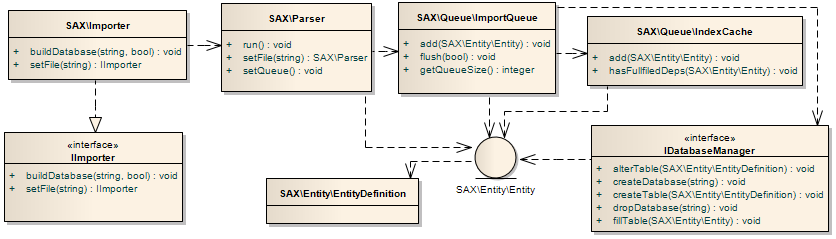
\includegraphics[scale=0.5]{figures/import.png}
\caption{Architektura importního skriptu}
\label{fig:queue}
\end{center}
\end{figure}


\section{Verzování databáze}
Požadavky na možnost verzování a definice schématu aktualizace dat vychází především ze zkušeností s provozem stávající verze Studentovy Berličky a problémů které jí pokusy o průběžný import dat v minulosti způsobily. Nemůžeme se totiž spolehnout na to, že data v rz.xml jsou stoprocentně konzistentní, nemůžeme se ani spolehnout že v rz.xml najdeme vždy všechna data, může se stát, že na pár dní z exportu vypadnou a zase se objeví.

Pro řešení těchto problémů jsem navrhl možnosti vytváření revizí databáze a vzájemné porovnávání rozdílů mezi nimi. Tím snadno odstraníme nebezpečí nekontrolované změny dat a jejich struktury a zároveň umožníme jejich zaktualizování v momentě, kdy je klientská aplikace na změny připravena, nebo když změny nepředstavují pro aplikaci problém.

\subsection{Aktualizace revize}
U každé revize lze na úrovni jednotlivých tabulek definovat, zda-li se má tabulka udržovat ve stavu v jakém byla při vytvoření revize, nebo ji má importní skript aktualizovat. Jsou k dispozici tyto možnosti:

\begin{itemize}
\item Neaktualizovat - V tomto případě zůstane tabulka stále stejná z okamžiku vytvoření revize.
\item Aktualizovat data - Tabulka bude automaticky po importování nové verze rz.xml naplněna aktuálními daty. Tato možnost bude doplněna navíc o údaj maximálního počtu změn v řádcích tabulky, pro které se ještě může provést aktualizace. V případě že bude tento počet překročen, bude upozorněn správce klientské aplikace. Stejně tak v případě že dojde ke změně struktury.
\item Aktualizovat vše - V takovém případě bude tato tabulka vždy přepsána aktuální verzí z posledního importu. Aplikace v takovém případě dostává stejná data jako by přistupovala přímo k "live" databázi a změny nejsou kontrolovány.
\end{itemize}

Definicí schématu \uv{aktualizovat pouze data} spolu s určením rozumného maximálního počtu změn v tabulce tak snadno dosáhneme potřebného promítnutí menších změn (například změna e-mailu) do revize, ale změny přes velký počet záznamů tabulky (jakým může být i dříve zmíněné přečíslování indexů) se do revize neprojeví dokud je administrátor klientské aplikace nezkontroluje a nepotvrdí.

Jednotlivé vytvořené jsou interně reprezentovány samostatnou databází, takovéto řešení je zřejmě tím nejvhodnějším pro tuto úlohu.

\subsection{Podmnožiny hlavní databáze}

Motivací pro navržení této funkce byl prostý fakt, že rz.xml obsahuje velké množství dat a vytvořená databáze tak zabírá zhruba 30MB. Ačkoli to není nijak závratně mnoho, je naprosto zbytečné, aby jednotlivé revize obsahovaly obraz celého rz.xml. Typická klientská aplikace totiž nepotřebuje všechna data, většinou si vystačí pouze s jejich zlomkem, třeba i jen s informacemi o jednom předmětu. Další výhodou je, že databázový stroj nebude muset prohledávat tisíce řádků, ale pouze malou část, a může tak výsledky vracet rychleji, což samozřejmě zrychlí i odpověď webové služby.

U vytvářené podmnožiny je velmi důležité, aby data v ní zůstala v konzistentní podobě a obsahovala všechny odkazované záznamy. Původní záměr byl takový, že si uživatel nadefinuje, které tabulky chce v revizi mít a při vytvoření budou automaticky rozpoznány veškeré závislosti které tabulky mají a to i například prostřednictvím takzvaných spojových tabulek. Řešení tohoto problému formou automatického rozpoznávání se ale ukázalo jako poměrně komplikovaný úkol a proto byl prozatím odložen.

Ve stávající verzi je tedy nutné vybrat do revize všechny tabulky, které revize bude obsahovat, včetně zmíněných spojových tabulek. Zároveň je možné odstranit sloupce cizích klíčů, které nechceme do revize přenést. Nicméně rozhraní a skript vytvářející revize odstranění cizích klíčů, jejich obrazy v revizi nebudou, nevyžadují, uživatel je pouze výrazně upozorněn na možnou nekonzistenci.

\section{Definice rozhraní}

Jak už bylo řečeno v požadavcích, aplikace umožňuje vlastní definici rozhraní webové služby SOAP. Uživatel má možnost definovat název procedury, její parametry včetně typů, způsob získání výsledků a návratový typ.

Zatímco implementace této funkčnosti v jiných, kompilovaných, jazycích by byla nejspíše velmi komplikovaná, pokud vůbec možná, v PHP lze tento problém řešit jednoduše a přímočaře využitím magické metody \texttt{call}. Tato metoda je volána vždy, pokud nad instancí třídy voláme metodu, která v ní není definována (ani v jejích předcích). Ve třídě, která se stará o obsluhu požadavků webové služby proto definujeme tuto metodu a obsloužení všech metod, které jsou uživatelsky definované je předáno právě jí. Procedury, která jsou pevnou součástí rozhraní služby (například pro identifikaci a autentizaci klienta) definujeme přímo v kódu třídy a PHP skript je zavolá přímo. V \texttt{call} tak máme jistotu že je volána jenom na uživatelsky definované procedury služby.

V současné verzi probíhá definice prostřednictvím formulářů na obrázcích \ref{fig:defOperace} a \ref{fig:defSQL}. V prvním formuláři uživatel definuje základní parametry procedury, ve druhém pak SQL dotaz, který se má při volání provést. SQL definice jedné operace se může lišit vůči jednotlivým revizím. 

\begin{figure}[h]
\begin{center}
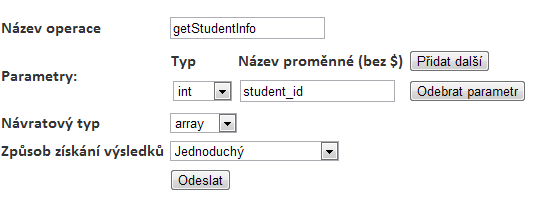
\includegraphics[scale=0.5]{figures/operace.png}
\caption{Formulář definice procedury webové služby}
\label{fig:defOperace}
\end{center}
\end{figure}

\begin{figure}[h]
\begin{center}
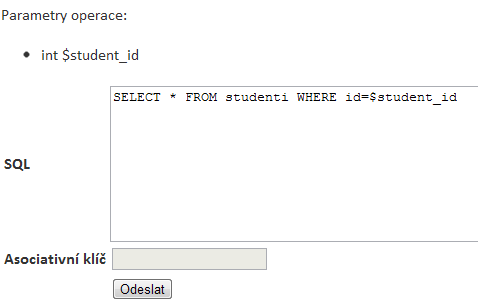
\includegraphics[scale=0.5]{figures/sql.png}
\caption{Formulář definice SQL dotazu}
\label{fig:defSQL}
\end{center}
\end{figure}

Výsledky je možné získávat ve třech podobách:
\begin{itemize}
\item Základní - jsou vráceny všechny výsledky v poli indexovaném od nuly.
\item Asociativní - podobně jako první možnost, ale pole je indexováno definovaným asociativním klíčem (nejčastěji primární klíč). Definice tohoto kliče se může lišit vůči jednotlivým revizím.
\item Jedno hodnotu - jak název napovídá, je vrácena jen jedna hodnota. Hodí se například pro použití s agregačními funkcemi SQL.
\end{itemize}

Pro otestování jednotlivých procedur služby je k dispozici testovací rozhraní.

Dalším krokem ve vývoji tohoto rozhraní bude generování potřebného SQL dotazu prostřednictvím uživatelsky přívětivějšího průvodce, bez nutnosti vypisovat samotný dotaz.


%*****************************************************************************
\chapter{Implementace}
Tato kapitola obsahuje postup nasazení aplikace na produkční server, popis jejích možností konfigurace a také příklad na klienta webové služby.
 
\section{Nasazení aplikace}
\subsection{Požadavky}
\begin{itemize}
\item Webový server s podporou PHP (doporučeným serverem, na kterém byla aplikace testována je Apache HTTPD 2.2 s PHP jako SAPI modulem).
\item PHP verze 5.3 nebo vyšší (aplikace využívá jmenné prostory a anonymní funkce). Jsou vyžadovány moduly PHP \textit{soap, curl, mbstring}.
\item Relační databázový stroj (doporučeno MySQL nebo PostgreSQL), a odpovídající modul PHP pro jeho podporu (možné použít PDO i nativní rozšíření).
\item Libovolný operační systém (testováno na platformě Windows a Debian GNU/Linux).
\end{itemize}
V případě použití jiného databázového stroje než MySQL je nutné doplnit do aplikace podporu implementaci rozhraní pro správu databází pod tímto RDBMS. Více viz kap. \ref{idatabasemanager}.

\subsection{Konfigurace}
Konfigurace aplikace je umístěna na místě standardním pro Nette aplikace - v souboru \textit{/app/config.ini}. Je velmi důležité, aby tento soubor zůstal nepřístupný pro přístup z webu, protože obsahuje citlivé informace. Z webu by měl být přístupný pouze adresář \textit{/www/}.

Při nasazování aplikace je nutné soubor config.ini vytvořit, distribuce obsahuje ve stejné složce připravený soubor config-default.ini, který obsahuje výchozí nastavení.

Konfigurační soubor Nette aplikace je rozdělen na části \textit{common, development} a \textit{production}. Jednotlivé sekce je možné v jiných \uv{dědit}, podobně jako třídy programu. K tomu se používá notace se špičatou závorkou (např. \texttt{[production < common]}). Uvedený příklad znamená, že sekce \textit{production} rozšiřuje sekci \textit{common}. Stejně jako u dědění tříd je možné přepsat nastavení nadřazené sekce, čehož se využívá například pro rozdílná nastavení připojení k databázi na vývojovém a produkčním serveru.

Konfigurační soubor obsahuje nastavení běhového prostředí aplikace a jejích služeb. Zde neuvádím všechny direktivy, které se v souboru vyskytují, ale jen ty které mohou být užitečné právě při nasazování aplikace. Zde neuvedené direktivy doporučuji neměnit, můžete tím znefunkčnit celou aplikaci!

Nastavení databáze:
\begin{itemize}
\item \textbf{database.driver} Databázový driver pro připojení. Lze použít jak nativní driver \textit{mysql, mysqli, pgsql} tak i \textit{pdo}.
\item \textbf{database.dsn} V případě použití PDO obsahuje DSN řetězec pro připojení k databázi. Při použití nativních ovladačů je ignorován.
\item \textbf{database.host} Adresa databázového stroje.
\item \textbf{database.username} Uživatelské jméno pro připojení
\item \textbf{database.password} Heslo pro připojení
\item \textbf{database.charset} Kódování znaků
\item \textbf{database.lazy} V případě nastavení této direktivy na TRUE je připojení k databázi vytvořeno až při provedení prvního dotazu.
\item \textbf{service.IDatabaseManager} Nastavení jména třídy, která implementuje připravené rozhraní \texttt{IDatabaseManager}, která se má použít pro práci s databází. Výchozí hodnotou je implementace \textit{MySQLDatabaseManager} pro databázový stroj MySQL.
\end{itemize}
Nastavení celé sekce \textit{database} vychází z API třídy \textit{DibiConnection}\cite{dibiconnection}, lze použít veškeré jeho možnosti. Na tomto místě bych také zdůraznil, že databázový uživatel musí mít práva pro vytváření, změnu a odstraňování databází a jejích tabulek.

Nastavení importního modulu:
\begin{itemize}
\item \textbf{xml.remoteURL} URL adresa vzdáleného zdroje, odkud se má rz.xml stáhnout.
\item \textbf{xml.login} Uživatelské jméno použité pro HTTP autentizaci.
\item \textbf{xml.password} Heslo použité pro HTTP autentizaci.
\item \textbf{xml.localRepository} Cesta k lokálnímu úložišti XML souborů.
\item \textbf{xml.liveDatabase} Název databáze, do které bude aktuální verze rz.xml převedena.
\end{itemize}


\section{Ukázková implementace klienta služby}
Protože webová služba umožňuje definici vlastního rozhraní služby, budu pro následující příklady předpokládat, že v aplikaci zadáno následující nastavení:
\begin{itemize}
\item Klient je identifikován jménem \uv{berlicka} a heslem \uv{test}.
\item Klient může načíst data z revize databáze pod názvem \uv{testing}.
\item Klient má definovánu jednu proceduru služby s názvem \textit{getStudentsInfo}, která má jako parametr pole studentských uživatelských jmen a vrací asociativní pole informací o studentech (z tabulky \textit{studenti}) indexované osobním ID.
\end{itemize}

Identifikace klientských aplikací probíhá zavoláním procedury \texttt{authenticate(jmeno, heslo)}. Je nutné volat tuto proceduru jako první, jinak služba vrací výjimku \textit{SoapFault}.

Další pevnou součástí rozhraní služby je \texttt{useRevision}, která slouží k výběru aktivní revize. Revizi lze bez problémů změnit během komunikace se službou, čili různá volání procedur mohou pracovat s různými revizemi. Pokud není před zavoláním nějaké procedury vybrána revize voláním \texttt{useRevision}, automaticky se použije revize nastavená pro klienta jako výchozí.

V distribuci PHP najdeme již zabudovanou podporu SOAP (přesněji je v rozšíření \textit{soap}, které je součástí distribuce), takže klienta vytvoříme snadno pomocí třídy SoapClient. Protože služba neposkytuje WSDL, je první parametr NULL a teprve druhým parametrem je určena adresa služby, tak jak to radí manuál PHP\cite{php:soap}. Nyní již slíbený příklad:
\begin{verbatim}
<?php

$soap = new SoapClient(NULL, array(
    "location" => 'http://URL_SERVERU/soap/',
    "uri" => 'http://URL_SERVERU/soap/'));
try {
    $soap->authenticate('berlicka', 'test');
    $soap->useRevision('testing');

    $return = $soap->getStudentsInfo(array('langeja1'));
    var_dump($return);
} catch (SoapFault $e) {
    echo $soap->getLastError();
}

?>
\end{verbatim}

Pokud vše proběhne v pořádku, obdržíme odpověď:

\begin{verbatim}
array(1) {
   355981000 => array(14) {
      "id" => "355981000" (9)
      "jmeno" => "Jan" (3)
      "login" => "langeja1" (8)
      "obor" => "Web a multimedia (bakalářský)" (32)
      "osoba_id" => "355981000" (9)
      "prijmeni" => "Langer" (6)
      "rocnik" => "3"
      "skupina" => "72" (2)
      "stlan_id" => "10201404" (8)
      "stud_email" => "langeja1@fel.cvut.cz" (20)
      "stud_id" => "15736704" (8)
      "titul" => NULL
      "titul_za" => NULL
   }
}
\end{verbatim}

\subsection{Zpracování chyb}
Jakákoliv chyba při zpracování požadavku (například v SQL dotazu, nesprávný formát parametrů nebo chybná identifikace) na straně serveru služby je indikována vyhozením výjimky. Na klientské straně se to projeví výjimkou \textit{SoapFault}, je tedy velmi vhodné ji zachytávat blokem try-catch. Ani po vyhození této speciální výjimky, ale nedojde k uzavření spojení a tak je možné zjistit textový popis chyby voláním procedury \texttt{getLastError()}. Stejný text je na straně serveru také zalogován a je možná ho najít v administračním rozhraní.


%*****************************************************************************
\chapter{Testování}
\section{Jednotkové testování}
Jednotkové (unit) testy slouží k testování samostatných částí aplikačního kódu - jednotek. Při použití oběktově orientovaného kódu je za jednotku většinou považována třída, a v rámci ní se obvykle testují jednotlivé metody. Jednotkové testování pomáhá udržovat při vývoji a pozdějším rozšiřování, zda-li jednou změnou nedošlo k chybnému chování programu na jiných místech. V PHP se pro vytváření těchto testů nejčastěji používá framework PHPUnit\cite{phpunit}.

Ačkoli co největší pokrytí kódu testy vede k jednodušší kontrole změn v aplikaci, je nutné mít na paměti, že samotné 100\% pokrytí kódu úspěšnými testy nutně neznamená, že je kód v pořádku, protože například nemusí být ošetřeny všechny vstupy. Spolupráce aplikace s okolními systémy (jakými může být databáze, nebo i uživatel) v podstatě znemožňuje 100\% pokrytí dosáhnout, neboť výstup některých částí kódu není deterministický vzhledem ke vstupu, závisí na kontextu.

V balíku aplikace jsou vytvořené testy pro třídy modelu a presenterů. Najdete je v adresáři \textit{/test}.

V tabulkách  \ref{tab:tab1} a \ref{tab:tab2} naleznete přehled testů a pokrytí kódu.

\begin{table}
\begin{center}
\begin{tabular}{|l|l|l|l|}
\hline
\textbf{Třída} & \textbf{Počet testů} & \textbf{Počet kontrol (assertions)} & \textbf{Pokrytí kódu} \\
\hline
\hline
Application & 5 & 7 & 80,49 \% \\
\hline
IndexDefinition & 1 & 3 & 86,96 \% \\
\hline
OperationSQL & 3 & 6 & 73,08 \% \\
\hline
Operation & 4 & 6 & 84,31 \% \\
\hline
UsersModel & 1 & 2 & 100 \% \\
\hline
\textbf{Celkem} & 14 & 20 & 84,97 \% \\
\hline
\end{tabular}
\end{center}
\caption{Testy modelových tříd}
\label{tab:tab1}
\end{table}

\begin{table}
\begin{center}
\begin{tabular}{|l|l|l|l|}
\hline
\textbf{Třída} & \textbf{Počet testů} & \textbf{Počet kontrol (assertions)} & \textbf{Pokrytí kódu} \\
\hline
\hline
AppPresenter & 5 & 5 & 68,75 \% \\
\hline
DefaultPresenter & 2 & 2 & 66,67 \% \\
\hline
KeyDefPresenter & 2 & 2 & 69,01 \% \\
\hline
LoginPresenter & 3 & 4 & 59,09 \% \\
\hline
OperationPresenter & 6 & 6 & 58,78 \% \\
\hline
RevisionPresenter & 8 & 11 & 54,29 \% \\
\hline
SoapTestPresenter & 4 & 4 & 60,26 \% \\
\hline
\textbf{Celkem} & 30 & 35 & 62,41 \% \\
\hline
\end{tabular}
\end{center}
\caption{Testy presenetrů}
\label{tab:tab2}
\end{table}


\section{Testování v provozu}

Během implementace jednotlivých funkčních celků aplikace docházelo průběžně k jejich testování tak, aby poskytovaly požadovanou funkčnost. Během zkouškového období v lednu a únoru 2011 dojde ještě k otestování aplikace propojením s Portálem pro podporu projektů v týmu, který je na FIT vyvíjen. Samotná aplikace by pak měla být spolu s tímto portálem uvedena do reálného provozu ze začátkem letního semestru 2010/2011. Poté se na aplikaci budou moci napojit i další aplikace, včetně nové Studentovy Berličky.

%*****************************************************************************
\chapter{Závěr}
V rámci této práce byl navržen a implementován relativně komplexní systém, který umožní aplikacím řízený přístup k datům o rozvrhu prostřednictvím standardního rozhraní SOAP. Aplikace takovéhoto typu samozřejmě není nikdy dokončena, vždy se dají najít věci, které by bylo vhodné doplnit, předělat nebo upravit. Jde o dlouhodobý projekt a hodlám se dalšímu rozvoji věnovat i po dokončení bakalářského studia.

Cílem této práce nebylo vyvinout univerzální systém, který obslouží jakoukoliv aplikaci, ani integrovat co největší množství datových zdrojů. Takovou úlohu by měla plnit aplikace KOS API (jeho připravovaná verze bude zpracovávat kromě rozvrhu i data Bílé knihy a připravují se další exporty). Cílem bylo vytvořit zdroj dat rozvrhu pro Studentovu Berličku a příbuzné aplikace (například již zmíněný systém pro podporu týmových projektů) a zároveň promítnout zkušenosti a odstranit problémy, které byly nalezeny v předchozích řešeních. Myslím, že výsledná aplikace tuto úlohu plní velmi dobře.

\section{Splnění cíle ze zadání}
Informace, která by jistě v závěru práce chybět neměla je, zda-li byly splněny všechny body úvodního zadání.
\begin{itemize}
\item \textit{Prozkoumejte možnosti, jak čerpat informace z informačního systému fakulty KOS} - Možnosti byly prozkoumány v kapitole \ref{popis}.
\item \textit{Proveďte analýzu potřeb Studentovy Berličky z hlediska možných importovatelných dat tak, aby zůstala zachována funkcionalita stávajícího řešení} - Výsledná aplikace využívá stejný zdroj dat jako původní řešení ve Studentově Berličce. Tato část zadání je tedy také splněna.
\item \textit{Na základě analýz navrhněte řešení importu informací o studentech, cvičeních a učitelích z informačních systému fakulty KOS do aplikace Studentova Berlička.} - Toto bylo primárním cílem celé práce. Splněno.
\item \textit{Implementovaný importní nástroj řádně otestujte.} Byly vytvořeny jednotkové testy a aplikace byla testována v průběhu vývoje. Otestování při propojení s reálnou aplikací a následně nasazení do provozu proběhne v nejbližší době.
\end{itemize}

%*****************************************************************************
% Seznam literatury je v samostatnem souboru reference.bib. Ten
% upravte dle vlastnich potreb, potom zpracujte (a do textu
% zapracujte) pomoci prikazu bibtex a nasledne pdflatex (nebo
% latex). Druhy z nich alespon 2x, aby se poresily odkazy.

% originally following specification for bibliography formating was used
%\bibliographystyle{abbrv}

% Here is an improvment by Petr Dlouhy (April 2010).
% It is mainly for supervisors who expect Czech fomrating rules for references
% Additional feature is live url addresses to sources from your pdf file
% It requires the file csplainnat.bst (included in this sample zipfile).

\bibliographystyle{csplainnat}

%bibliographystyle{plain}
%\bibliographystyle{psc}
{
%JZ: 11.12.2008 Kdo chce mit v techto ukazkovych odkazech take odkaz na CSTeX:
%\def\CS{$\cal C\kern-0.1667em\lower.5ex\hbox{$\cal S$}\kern-0.075em $}
\bibliography{reference}
}

% M. Dušek radi:
%\bibliographystyle{alpha}
% kdy citace ma tvar [AutorRok] (napriklad [Cook97]). Sice to asi neni  podle ceske normy (BTW BibTeX stejne neodpovida ceske norme), ale je to nejprehlednejsi.
% 3.5.2009 JZ polemizuje: BibTeX neobvinujte, napiste a poskytnete nam styl (.bst) splnujici citacni normu CSN/ISO.

%*****************************************************************************
%*****************************************************************************
\appendix


%*****************************************************************************
\chapter{Seznam použitých zkratek}

\begin{description}
\item[API] - Application Programming Interface 
\item[BSD] - Berkeley Software Distribution
\item[CLI] - Command Line Interface
\item[ČVUT] - České vysoké učení technické
\item[DBMS] - Database Management System
\item[DOM] - Document Object Model
\item[DRY] - Don't repeat yourself
\item[EUNIS] - European UNiversity Information Systems
\item[FEL] - Fakulta elektrotechnická
\item[FIT] - Fakulta informačních technologií
\item[FS] - Fakulta strojní
\item[FTP] - File Transfer Protocol
\item[GNU] - GNU's not Unix (rekurzivní zkratka)
\item[GPL] - General Public License
\item[GUI] - Graphical User Interface
\item[HTTP] - Hypertext Transfer Protocol
\item[HTTPD] - Hypertext Transfer Protocol Daemon
\item[IS] - Informační systém
\item[KISS] - Keep It Short and Simple
\item[KOS] - Komponenta Studium
\item[MVC] - Model View Controller
\item[MVP] - Model View Presenter
\item[OOP] - Object-oriented programming
\item[PDO] - PHP Data Objects
\item[RDBMS] - Relational Database Mangement System
\item[REST] - Representational State Transfer
\item[RPC] - Remote Procedure Call
\item[SAPI] - Server Application Programming Interface
\item[SAX] - Simple API for XML
\item[SMTP] - Simple Mail Transfer Protocol
\item[SOAP] - Simple Object Access Protocol
\item[SQL] - Structured Query Language
\item[URL] - Uniform Resource Locator
\item[VIC] - Výpočení a Informační Centrum ČVUT
\item[WS] - Web Services
\item[WSDL] - Web Services Description Language
\item[WWW] - World Wide Web
\item[XML] - Extensible Markup Language
\item[XSLT] - Extensible Stylesheet Language Transformations
\end{description}

%*****************************************************************************
\chapter{Obsah přiloženého CD}
\textbf{\large Tato příloha je povinná pro každou práci. Každá práce musí totiž obsahovat přiložené CD. Viz dále.}

Může vypadat například takto. Váš seznam samozřejmě bude odpovídat typu vaší práce. (viz cite{infodp}):

\begin{figure}[h]
\begin{center}
%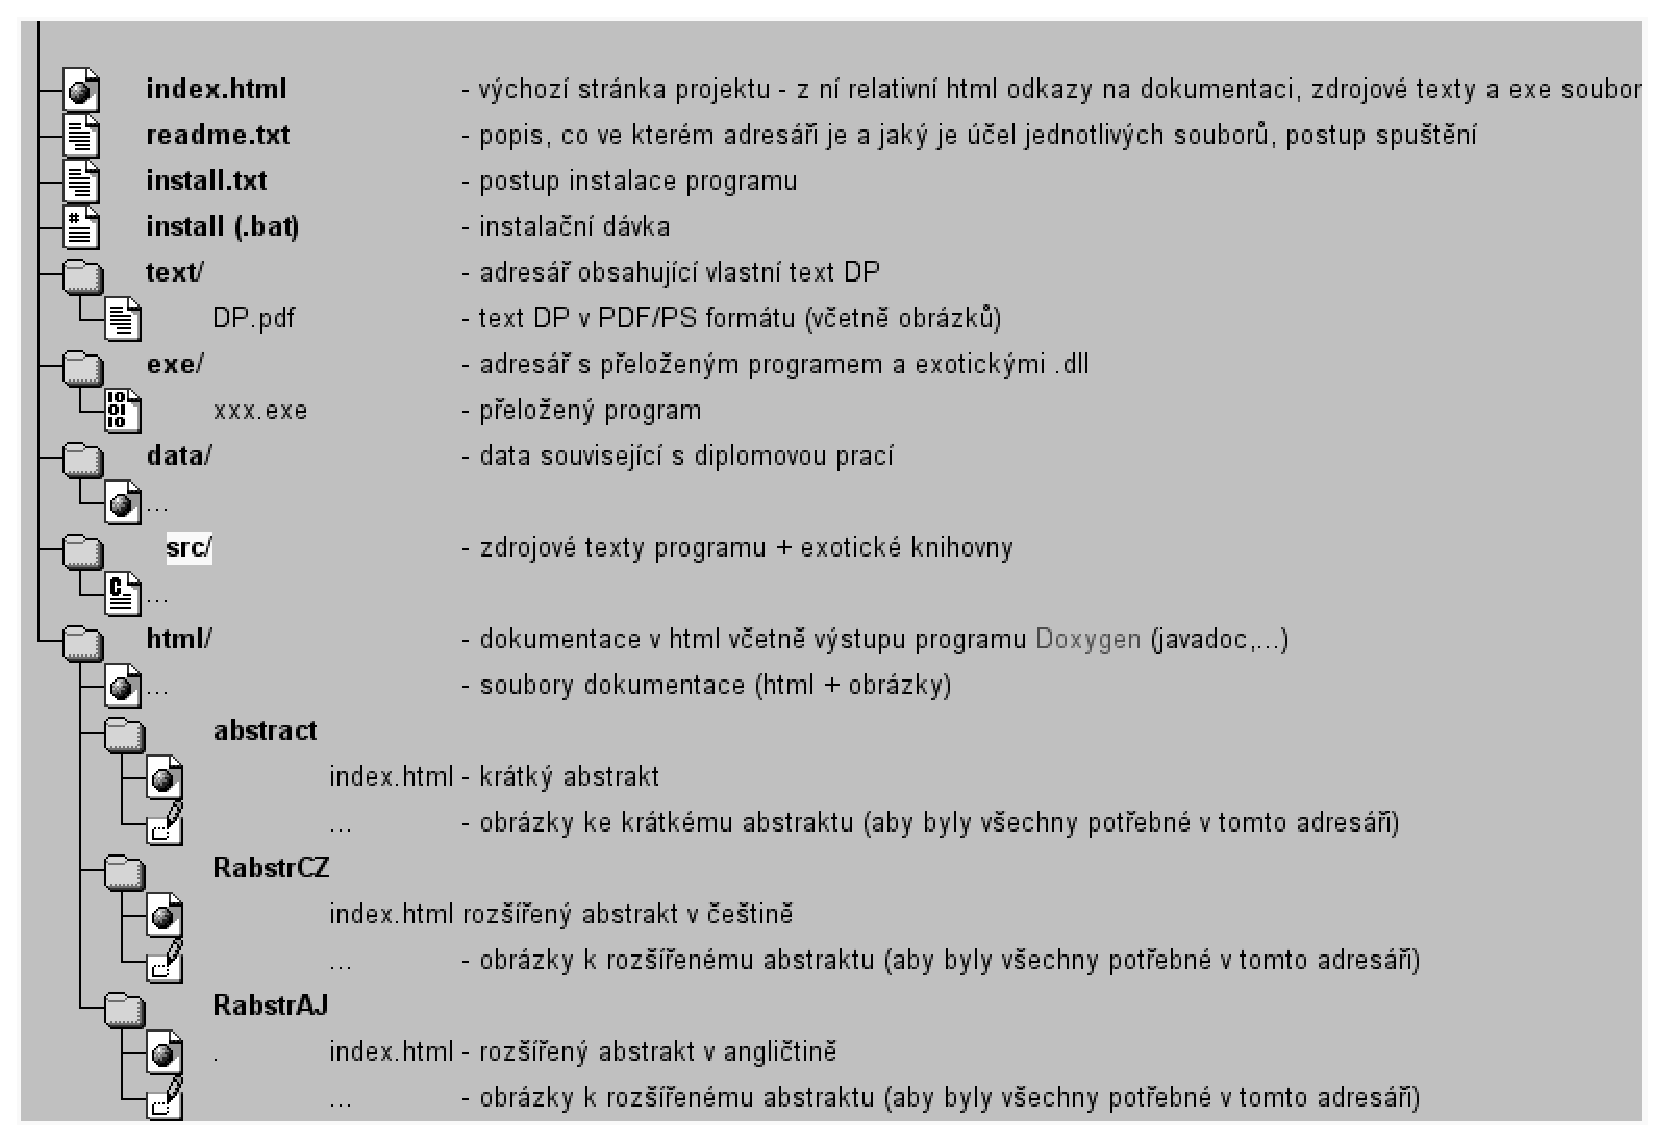
\includegraphics[width=14cm]{figures/seznamcd}
\caption{Seznam přiloženého CD --- příklad}
%\label{fig:seznamcd}
\end{center}
\end{figure}

Na GNU/Linuxu si strukturu přiloženého CD můžete snadno vyrobit příkazem:\\ 
\verb|$ tree . >tree.txt|\\
Ve vzniklém souboru pak stačí pouze doplnit komentáře.

Z \textbf{README.TXT} (případne index.html apod.)  musí být rovněž zřejmé, jak programy instalovat, spouštět a jaké požadavky mají tyto programy na hardware.

Adresář \textbf{text}  musí obsahovat soubor s vlastním textem práce v PDF nebo PS formátu, který bude později použit pro prezentaci diplomové práce na WWW.

\end{document}
